\documentclass[]{article}

\usepackage{deauthor}


% \usepackage{amsmath}
% \usepackage{graphicx}
% \usepackage{wrapfig}
% \usepackage{xspace}
% \usepackage{xcolor}
% \usepackage{colortbl}
% \usepackage{titlesec}
% \usepackage{hyperref}
% \usepackage{cleveref}
% \usepackage{ulem}
% \usepackage[numbers,sort&compress]{natbib}
% \usepackage{tcolorbox}

% \newcommand{\ie}[0]{\textit{i.e.}}
% \newcommand{\eg}[0]{\textit{e.g.}}
% \newcommand{\etc}[0]{\textit{etc.}}
% \newcommand{\wrt}[0]{\textit{w.r.t.}}
% \newcommand{\aka}[0]{\textit{a.k.a.}}

% \newcommand{\ours}[0]{\texttt{KLC}\xspace}
% \newcommand{\todo}[1]{\textcolor{red}{TODO: #1}}
% \newcommand{\carl}[1]{\textcolor{cyan}{Carl: #1}}

% % \newcommand{\modify}[1]{\textcolor{blue}{#1}}
% \DeclareRobustCommand{\modify}[1]{{\color{blue}#1}}  
% \newcommand{\delete}[1]{\textcolor{red}{\sout{#1}}}
% % \DeclareRobustCommand{\modify}[1]{{\color{blue}#1}}  
% % change into the following to hide
% %\newcommand{\modify}[1]{#1}
% %\newcommand{\delete}[1]{}


% %%%%% NEW MATH DEFINITIONS %%%%%

\usepackage{amsmath,amsfonts,bm}

% Mark sections of captions for referring to divisions of figures
\newcommand{\figleft}{{\em (Left)}}
\newcommand{\figcenter}{{\em (Center)}}
\newcommand{\figright}{{\em (Right)}}
\newcommand{\figtop}{{\em (Top)}}
\newcommand{\figbottom}{{\em (Bottom)}}
\newcommand{\captiona}{{\em (a)}}
\newcommand{\captionb}{{\em (b)}}
\newcommand{\captionc}{{\em (c)}}
\newcommand{\captiond}{{\em (d)}}

% Highlight a newly defined term
\newcommand{\newterm}[1]{{\bf #1}}


% Figure reference, lower-case.
\def\figref#1{figure~\ref{#1}}
% Figure reference, capital. For start of sentence
\def\Figref#1{Figure~\ref{#1}}
\def\twofigref#1#2{figures \ref{#1} and \ref{#2}}
\def\quadfigref#1#2#3#4{figures \ref{#1}, \ref{#2}, \ref{#3} and \ref{#4}}
% Section reference, lower-case.
\def\secref#1{section~\ref{#1}}
% Section reference, capital.
\def\Secref#1{Section~\ref{#1}}
% Reference to two sections.
\def\twosecrefs#1#2{sections \ref{#1} and \ref{#2}}
% Reference to three sections.
\def\secrefs#1#2#3{sections \ref{#1}, \ref{#2} and \ref{#3}}
% Reference to an equation, lower-case.
\def\eqref#1{equation~\ref{#1}}
% Reference to an equation, upper case
\def\Eqref#1{Equation~\ref{#1}}
% A raw reference to an equation---avoid using if possible
\def\plaineqref#1{\ref{#1}}
% Reference to a chapter, lower-case.
\def\chapref#1{chapter~\ref{#1}}
% Reference to an equation, upper case.
\def\Chapref#1{Chapter~\ref{#1}}
% Reference to a range of chapters
\def\rangechapref#1#2{chapters\ref{#1}--\ref{#2}}
% Reference to an algorithm, lower-case.
\def\algref#1{algorithm~\ref{#1}}
% Reference to an algorithm, upper case.
\def\Algref#1{Algorithm~\ref{#1}}
\def\twoalgref#1#2{algorithms \ref{#1} and \ref{#2}}
\def\Twoalgref#1#2{Algorithms \ref{#1} and \ref{#2}}
% Reference to a part, lower case
\def\partref#1{part~\ref{#1}}
% Reference to a part, upper case
\def\Partref#1{Part~\ref{#1}}
\def\twopartref#1#2{parts \ref{#1} and \ref{#2}}

\def\ceil#1{\lceil #1 \rceil}
\def\floor#1{\lfloor #1 \rfloor}
\def\1{\bm{1}}
\newcommand{\train}{\mathcal{D}}
\newcommand{\valid}{\mathcal{D_{\mathrm{valid}}}}
\newcommand{\test}{\mathcal{D_{\mathrm{test}}}}

\def\eps{{\epsilon}}


% Random variables
\def\reta{{\textnormal{$\eta$}}}
\def\ra{{\textnormal{a}}}
\def\rb{{\textnormal{b}}}
\def\rc{{\textnormal{c}}}
\def\rd{{\textnormal{d}}}
\def\re{{\textnormal{e}}}
\def\rf{{\textnormal{f}}}
\def\rg{{\textnormal{g}}}
\def\rh{{\textnormal{h}}}
\def\ri{{\textnormal{i}}}
\def\rj{{\textnormal{j}}}
\def\rk{{\textnormal{k}}}
\def\rl{{\textnormal{l}}}
% rm is already a command, just don't name any random variables m
\def\rn{{\textnormal{n}}}
\def\ro{{\textnormal{o}}}
\def\rp{{\textnormal{p}}}
\def\rq{{\textnormal{q}}}
\def\rr{{\textnormal{r}}}
\def\rs{{\textnormal{s}}}
\def\rt{{\textnormal{t}}}
\def\ru{{\textnormal{u}}}
\def\rv{{\textnormal{v}}}
\def\rw{{\textnormal{w}}}
\def\rx{{\textnormal{x}}}
\def\ry{{\textnormal{y}}}
\def\rz{{\textnormal{z}}}

% Random vectors
\def\rvepsilon{{\mathbf{\epsilon}}}
\def\rvtheta{{\mathbf{\theta}}}
\def\rva{{\mathbf{a}}}
\def\rvb{{\mathbf{b}}}
\def\rvc{{\mathbf{c}}}
\def\rvd{{\mathbf{d}}}
\def\rve{{\mathbf{e}}}
\def\rvf{{\mathbf{f}}}
\def\rvg{{\mathbf{g}}}
\def\rvh{{\mathbf{h}}}
\def\rvu{{\mathbf{i}}}
\def\rvj{{\mathbf{j}}}
\def\rvk{{\mathbf{k}}}
\def\rvl{{\mathbf{l}}}
\def\rvm{{\mathbf{m}}}
\def\rvn{{\mathbf{n}}}
\def\rvo{{\mathbf{o}}}
\def\rvp{{\mathbf{p}}}
\def\rvq{{\mathbf{q}}}
\def\rvr{{\mathbf{r}}}
\def\rvs{{\mathbf{s}}}
\def\rvt{{\mathbf{t}}}
\def\rvu{{\mathbf{u}}}
\def\rvv{{\mathbf{v}}}
\def\rvw{{\mathbf{w}}}
\def\rvx{{\mathbf{x}}}
\def\rvy{{\mathbf{y}}}
\def\rvz{{\mathbf{z}}}

% Elements of random vectors
\def\erva{{\textnormal{a}}}
\def\ervb{{\textnormal{b}}}
\def\ervc{{\textnormal{c}}}
\def\ervd{{\textnormal{d}}}
\def\erve{{\textnormal{e}}}
\def\ervf{{\textnormal{f}}}
\def\ervg{{\textnormal{g}}}
\def\ervh{{\textnormal{h}}}
\def\ervi{{\textnormal{i}}}
\def\ervj{{\textnormal{j}}}
\def\ervk{{\textnormal{k}}}
\def\ervl{{\textnormal{l}}}
\def\ervm{{\textnormal{m}}}
\def\ervn{{\textnormal{n}}}
\def\ervo{{\textnormal{o}}}
\def\ervp{{\textnormal{p}}}
\def\ervq{{\textnormal{q}}}
\def\ervr{{\textnormal{r}}}
\def\ervs{{\textnormal{s}}}
\def\ervt{{\textnormal{t}}}
\def\ervu{{\textnormal{u}}}
\def\ervv{{\textnormal{v}}}
\def\ervw{{\textnormal{w}}}
\def\ervx{{\textnormal{x}}}
\def\ervy{{\textnormal{y}}}
\def\ervz{{\textnormal{z}}}

% Random matrices
\def\rmA{{\mathbf{A}}}
\def\rmB{{\mathbf{B}}}
\def\rmC{{\mathbf{C}}}
\def\rmD{{\mathbf{D}}}
\def\rmE{{\mathbf{E}}}
\def\rmF{{\mathbf{F}}}
\def\rmG{{\mathbf{G}}}
\def\rmH{{\mathbf{H}}}
\def\rmI{{\mathbf{I}}}
\def\rmJ{{\mathbf{J}}}
\def\rmK{{\mathbf{K}}}
\def\rmL{{\mathbf{L}}}
\def\rmM{{\mathbf{M}}}
\def\rmN{{\mathbf{N}}}
\def\rmO{{\mathbf{O}}}
\def\rmP{{\mathbf{P}}}
\def\rmQ{{\mathbf{Q}}}
\def\rmR{{\mathbf{R}}}
\def\rmS{{\mathbf{S}}}
\def\rmT{{\mathbf{T}}}
\def\rmU{{\mathbf{U}}}
\def\rmV{{\mathbf{V}}}
\def\rmW{{\mathbf{W}}}
\def\rmX{{\mathbf{X}}}
\def\rmY{{\mathbf{Y}}}
\def\rmZ{{\mathbf{Z}}}

% Elements of random matrices
\def\ermA{{\textnormal{A}}}
\def\ermB{{\textnormal{B}}}
\def\ermC{{\textnormal{C}}}
\def\ermD{{\textnormal{D}}}
\def\ermE{{\textnormal{E}}}
\def\ermF{{\textnormal{F}}}
\def\ermG{{\textnormal{G}}}
\def\ermH{{\textnormal{H}}}
\def\ermI{{\textnormal{I}}}
\def\ermJ{{\textnormal{J}}}
\def\ermK{{\textnormal{K}}}
\def\ermL{{\textnormal{L}}}
\def\ermM{{\textnormal{M}}}
\def\ermN{{\textnormal{N}}}
\def\ermO{{\textnormal{O}}}
\def\ermP{{\textnormal{P}}}
\def\ermQ{{\textnormal{Q}}}
\def\ermR{{\textnormal{R}}}
\def\ermS{{\textnormal{S}}}
\def\ermT{{\textnormal{T}}}
\def\ermU{{\textnormal{U}}}
\def\ermV{{\textnormal{V}}}
\def\ermW{{\textnormal{W}}}
\def\ermX{{\textnormal{X}}}
\def\ermY{{\textnormal{Y}}}
\def\ermZ{{\textnormal{Z}}}

% Vectors
\def\vzero{{\bm{0}}}
\def\vone{{\bm{1}}}
\def\vmu{{\bm{\mu}}}
\def\vtheta{{\bm{\theta}}}
\def\va{{\bm{a}}}
\def\vb{{\bm{b}}}
\def\vc{{\bm{c}}}
\def\vd{{\bm{d}}}
\def\ve{{\bm{e}}}
\def\vf{{\bm{f}}}
\def\vg{{\bm{g}}}
\def\vh{{\bm{h}}}
\def\vi{{\bm{i}}}
\def\vj{{\bm{j}}}
\def\vk{{\bm{k}}}
\def\vl{{\bm{l}}}
\def\vm{{\bm{m}}}
\def\vn{{\bm{n}}}
\def\vo{{\bm{o}}}
\def\vp{{\bm{p}}}
\def\vq{{\bm{q}}}
\def\vr{{\bm{r}}}
\def\vs{{\bm{s}}}
\def\vt{{\bm{t}}}
\def\vu{{\bm{u}}}
\def\vv{{\bm{v}}}
\def\vw{{\bm{w}}}
\def\vx{{\bm{x}}}
\def\vy{{\bm{y}}}
\def\vz{{\bm{z}}}

% Elements of vectors
\def\evalpha{{\alpha}}
\def\evbeta{{\beta}}
\def\evepsilon{{\epsilon}}
\def\evlambda{{\lambda}}
\def\evomega{{\omega}}
\def\evmu{{\mu}}
\def\evpsi{{\psi}}
\def\evsigma{{\sigma}}
\def\evtheta{{\theta}}
\def\eva{{a}}
\def\evb{{b}}
\def\evc{{c}}
\def\evd{{d}}
\def\eve{{e}}
\def\evf{{f}}
\def\evg{{g}}
\def\evh{{h}}
\def\evi{{i}}
\def\evj{{j}}
\def\evk{{k}}
\def\evl{{l}}
\def\evm{{m}}
\def\evn{{n}}
\def\evo{{o}}
\def\evp{{p}}
\def\evq{{q}}
\def\evr{{r}}
\def\evs{{s}}
\def\evt{{t}}
\def\evu{{u}}
\def\evv{{v}}
\def\evw{{w}}
\def\evx{{x}}
\def\evy{{y}}
\def\evz{{z}}

% Matrix
\def\mA{{\bm{A}}}
\def\mB{{\bm{B}}}
\def\mC{{\bm{C}}}
\def\mD{{\bm{D}}}
\def\mE{{\bm{E}}}
\def\mF{{\bm{F}}}
\def\mG{{\bm{G}}}
\def\mH{{\bm{H}}}
\def\mI{{\bm{I}}}
\def\mJ{{\bm{J}}}
\def\mK{{\bm{K}}}
\def\mL{{\bm{L}}}
\def\mM{{\bm{M}}}
\def\mN{{\bm{N}}}
\def\mO{{\bm{O}}}
\def\mP{{\bm{P}}}
\def\mQ{{\bm{Q}}}
\def\mR{{\bm{R}}}
\def\mS{{\bm{S}}}
\def\mT{{\bm{T}}}
\def\mU{{\bm{U}}}
\def\mV{{\bm{V}}}
\def\mW{{\bm{W}}}
\def\mX{{\bm{X}}}
\def\mY{{\bm{Y}}}
\def\mZ{{\bm{Z}}}
\def\mBeta{{\bm{\beta}}}
\def\mPhi{{\bm{\Phi}}}
\def\mLambda{{\bm{\Lambda}}}
\def\mSigma{{\bm{\Sigma}}}

% Tensor
\DeclareMathAlphabet{\mathsfit}{\encodingdefault}{\sfdefault}{m}{sl}
\SetMathAlphabet{\mathsfit}{bold}{\encodingdefault}{\sfdefault}{bx}{n}
\newcommand{\tens}[1]{\bm{\mathsfit{#1}}}
\def\tA{{\tens{A}}}
\def\tB{{\tens{B}}}
\def\tC{{\tens{C}}}
\def\tD{{\tens{D}}}
\def\tE{{\tens{E}}}
\def\tF{{\tens{F}}}
\def\tG{{\tens{G}}}
\def\tH{{\tens{H}}}
\def\tI{{\tens{I}}}
\def\tJ{{\tens{J}}}
\def\tK{{\tens{K}}}
\def\tL{{\tens{L}}}
\def\tM{{\tens{M}}}
\def\tN{{\tens{N}}}
\def\tO{{\tens{O}}}
\def\tP{{\tens{P}}}
\def\tQ{{\tens{Q}}}
\def\tR{{\tens{R}}}
\def\tS{{\tens{S}}}
\def\tT{{\tens{T}}}
\def\tU{{\tens{U}}}
\def\tV{{\tens{V}}}
\def\tW{{\tens{W}}}
\def\tX{{\tens{X}}}
\def\tY{{\tens{Y}}}
\def\tZ{{\tens{Z}}}


% Graph
\def\gA{{\mathcal{A}}}
\def\gB{{\mathcal{B}}}
\def\gC{{\mathcal{C}}}
\def\gD{{\mathcal{D}}}
\def\gE{{\mathcal{E}}}
\def\gF{{\mathcal{F}}}
\def\gG{{\mathcal{G}}}
\def\gH{{\mathcal{H}}}
\def\gI{{\mathcal{I}}}
\def\gJ{{\mathcal{J}}}
\def\gK{{\mathcal{K}}}
\def\gL{{\mathcal{L}}}
\def\gM{{\mathcal{M}}}
\def\gN{{\mathcal{N}}}
\def\gO{{\mathcal{O}}}
\def\gP{{\mathcal{P}}}
\def\gQ{{\mathcal{Q}}}
\def\gR{{\mathcal{R}}}
\def\gS{{\mathcal{S}}}
\def\gT{{\mathcal{T}}}
\def\gU{{\mathcal{U}}}
\def\gV{{\mathcal{V}}}
\def\gW{{\mathcal{W}}}
\def\gX{{\mathcal{X}}}
\def\gY{{\mathcal{Y}}}
\def\gZ{{\mathcal{Z}}}

% Sets
\def\sA{{\mathbb{A}}}
\def\sB{{\mathbb{B}}}
\def\sC{{\mathbb{C}}}
\def\sD{{\mathbb{D}}}
% Don't use a set called E, because this would be the same as our symbol
% for expectation.
\def\sF{{\mathbb{F}}}
\def\sG{{\mathbb{G}}}
\def\sH{{\mathbb{H}}}
\def\sI{{\mathbb{I}}}
\def\sJ{{\mathbb{J}}}
\def\sK{{\mathbb{K}}}
\def\sL{{\mathbb{L}}}
\def\sM{{\mathbb{M}}}
\def\sN{{\mathbb{N}}}
\def\sO{{\mathbb{O}}}
\def\sP{{\mathbb{P}}}
\def\sQ{{\mathbb{Q}}}
\def\sR{{\mathbb{R}}}
\def\sS{{\mathbb{S}}}
\def\sT{{\mathbb{T}}}
\def\sU{{\mathbb{U}}}
\def\sV{{\mathbb{V}}}
\def\sW{{\mathbb{W}}}
\def\sX{{\mathbb{X}}}
\def\sY{{\mathbb{Y}}}
\def\sZ{{\mathbb{Z}}}

% Entries of a matrix
\def\emLambda{{\Lambda}}
\def\emA{{A}}
\def\emB{{B}}
\def\emC{{C}}
\def\emD{{D}}
\def\emE{{E}}
\def\emF{{F}}
\def\emG{{G}}
\def\emH{{H}}
\def\emI{{I}}
\def\emJ{{J}}
\def\emK{{K}}
\def\emL{{L}}
\def\emM{{M}}
\def\emN{{N}}
\def\emO{{O}}
\def\emP{{P}}
\def\emQ{{Q}}
\def\emR{{R}}
\def\emS{{S}}
\def\emT{{T}}
\def\emU{{U}}
\def\emV{{V}}
\def\emW{{W}}
\def\emX{{X}}
\def\emY{{Y}}
\def\emZ{{Z}}
\def\emSigma{{\Sigma}}

% entries of a tensor
% Same font as tensor, without \bm wrapper
\newcommand{\etens}[1]{\mathsfit{#1}}
\def\etLambda{{\etens{\Lambda}}}
\def\etA{{\etens{A}}}
\def\etB{{\etens{B}}}
\def\etC{{\etens{C}}}
\def\etD{{\etens{D}}}
\def\etE{{\etens{E}}}
\def\etF{{\etens{F}}}
\def\etG{{\etens{G}}}
\def\etH{{\etens{H}}}
\def\etI{{\etens{I}}}
\def\etJ{{\etens{J}}}
\def\etK{{\etens{K}}}
\def\etL{{\etens{L}}}
\def\etM{{\etens{M}}}
\def\etN{{\etens{N}}}
\def\etO{{\etens{O}}}
\def\etP{{\etens{P}}}
\def\etQ{{\etens{Q}}}
\def\etR{{\etens{R}}}
\def\etS{{\etens{S}}}
\def\etT{{\etens{T}}}
\def\etU{{\etens{U}}}
\def\etV{{\etens{V}}}
\def\etW{{\etens{W}}}
\def\etX{{\etens{X}}}
\def\etY{{\etens{Y}}}
\def\etZ{{\etens{Z}}}

% The true underlying data generating distribution
\newcommand{\pdata}{p_{\rm{data}}}
% The empirical distribution defined by the training set
\newcommand{\ptrain}{\hat{p}_{\rm{data}}}
\newcommand{\Ptrain}{\hat{P}_{\rm{data}}}
% The model distribution
\newcommand{\pmodel}{p_{\rm{model}}}
\newcommand{\Pmodel}{P_{\rm{model}}}
\newcommand{\ptildemodel}{\tilde{p}_{\rm{model}}}
% Stochastic autoencoder distributions
\newcommand{\pencode}{p_{\rm{encoder}}}
\newcommand{\pdecode}{p_{\rm{decoder}}}
\newcommand{\precons}{p_{\rm{reconstruct}}}

\newcommand{\laplace}{\mathrm{Laplace}} % Laplace distribution

\newcommand{\E}{\mathbb{E}}
\newcommand{\Ls}{\mathcal{L}}
\newcommand{\R}{\mathbb{R}}
\newcommand{\emp}{\tilde{p}}
\newcommand{\lr}{\alpha}
\newcommand{\reg}{\lambda}
\newcommand{\rect}{\mathrm{rectifier}}
\newcommand{\softmax}{\mathrm{softmax}}
\newcommand{\sigmoid}{\sigma}
\newcommand{\softplus}{\zeta}
\newcommand{\KL}{D_{\mathrm{KL}}}
\newcommand{\Var}{\mathrm{Var}}
\newcommand{\standarderror}{\mathrm{SE}}
\newcommand{\Cov}{\mathrm{Cov}}
% Wolfram Mathworld says $L^2$ is for function spaces and $\ell^2$ is for vectors
% But then they seem to use $L^2$ for vectors throughout the site, and so does
% wikipedia.
\newcommand{\normlzero}{L^0}
\newcommand{\normlone}{L^1}
\newcommand{\normltwo}{L^2}
\newcommand{\normlp}{L^p}
\newcommand{\normmax}{L^\infty}

\newcommand{\parents}{Pa} % See usage in notation.tex. Chosen to match Daphne's book.

\DeclareMathOperator*{\argmax}{arg\,max}
\DeclareMathOperator*{\argmin}{arg\,min}

\DeclareMathOperator{\sign}{sign}
\DeclareMathOperator{\Tr}{Tr}
\let\ab\allowbreak


\begin{document}

\title{Knowledge Graph and Large Language Model Co-learning via Structure-oriented \mbox{Retrieval Augmented Generation}}
%\title{KG and LLM Co-learning via Structure-oriented RAG}

\author{Carl Yang\thanks{Corresponding author (j.carlyang@emory.edu); Department of Computer Science, Emory University, Atlanta, GA 30322, USA}, Ran Xu, Linhao Luo, Shirui Pan}

\maketitle

\begin{abstract}
Recent years have witnessed major technical breakthroughs in AI-- facilitated by tremendous data and high-performance computers, large language models (LLMs) have brought disruptive progress to information technology from accessing data to performing analysis. While demonstrating unprecedented capabilities, LLMs have been found unreliable in tasks requiring factual knowledge and rigorous reasoning. Despite recent works discussing the hallucination problem of LLMs, systematic studies on empowering LLMs with the ability to plan, reason, and ground with explicit knowledge are still lacking. 
On the other hand, real-world data are enormous and complex, coming from different sources and bearing various modalities. Data professionals have spent tremendous efforts collecting and curating countless datasets with different schemas and standards. Transforming the separate datasets into unified knowledge graphs (KGs) can facilitate their integrative analysis and utilization, but these processes would often require strong domain expertise and significant human labor. 
{In this paper, we discuss recent progress and promise in the co-learning of KGs and LLMs, through LLM-aided KG construction, KG-guided LLM enhancement, and knowledge-aware multi-agent federation, particularly emphasizing a structure-oriented retrieval augmented generation (SRAG) paradigm, towards fully utilizing the value of complex data, unleashing the power of generative models, and expediting next-generation trustworthy AI.} 
\end{abstract}


\section{Introduction}

%llm
Large language models (LLMs) have reshaped AI research and implementations, with unprecedented capabilities widely shown in various language-related tasks \cite{achiam2023gpt, leiter2024chatgpt, reid2024gemini, adler2024nemotron, jiang2023mistral, touvron2023llama, team2024gemma}, bringing humans ever close to general AI \cite{brown2020language, bubeck2023sparks, ge2024openagi}.
Recent research on multi-agent systems has further magnified LLMs' advantages of {\textit{broad knowledge}, \textit{language comprehension}, and \textit{generalizability}} through conversational collaborations, showing strong promise for further human-model collaboration for critical applications \cite{bankes2002agent, bai2022constitutional, bonabeau2002agent, li2023camel, wu2024autogen}.
Recent studies have also revealed the limitations of LLMs regarding their {\textit{lack of planning} \cite{hu2023large, mousavi2024your, yadkori2024believe, asai2024selfrag,yu2024rankrag}, \textit{fuzzy inference} \cite{liu2023evaluating, zhu2023dyval, zhuo2024roles, yuan2024back, wang2023boosting}, and \textit{hallucination} \cite{ji2023survey, bai2024hallucination, tonmoy2024comprehensive, maynez2020faithfulness, xiao2021hallucination, farquhar2024detecting, ji2023towards, chen2024inside}}. Specifically, in many real-world application scenarios, the lack of accurate planning can be caused by the lack of access to high-quality domain knowledge, especially the rapidly evolving new knowledge; the fuzzy inference nature can lead to difficulties in conducting reliable comprehension and stable predictions for complex questions; and hallucination creating factual errors and misinformation can cause fatal and life-threatening problems in critical applications \cite{wornow2023shaky, shen2023chatgpt, pal2023med, xu2024simrag, panagoulias2024evaluating, gu2024medvh}.
% motivations for multi-agent systems, black-box nature of LLMs makes it hard to share data/resource

%kg
Knowledge graphs (KGs) have been widely studied across academia and industry, due to their advantages in {\textit{storing accurate knowledge}, \textit{facilitating explicit inference}, and \textit{allowing easy editing of the knowledge} \cite{hogan2021knowledge, ji2021survey, wang2017knowledge, zou2020survey}}.
{However, the creation of KGs relies much on the \textit{standardization of data}, which requires significant schematic designs and human efforts.}
In many application domains, researchers and professionals have spent decades collecting, processing, and curating various types of data towards the construction of KGs \cite{cui2023review, su2023biomedical, cornet2008forty, santos2020clinical, harrison2021icd, lipscomb2000medical, bodenreider2004unified, xu2020building, li2020real, lv2023tcmbank}, which are widely used to support downstream application such as search and ranking \cite{xiong2017explicit, liu2018entity, vu2019capsule}, user modeling and recommendation \cite{wang2019kgat, wang2021learning, yang2022knowledge}, basic science research \cite{feng2023genomickb, shao2022knowledge, quan2023aimedgraph, zhang2021discovering, li2022prediction, jeong2022intelligent}, healthcare \cite{xu2023seqcare,jiang2024graphcare,xu2024ram} and education \cite{chen2018knowedu, rizun2019knowledge}. 
{Nevertheless, KGs still suffer from \textit{incomplete knowledge coverage}, due to the stringent requirements on data standardization and limited data volumes compared to unstructured data in the wild, while specific algorithms are often needed to fill \textit{their gaps to applications}}.
Moreover, real-world data are noisy and complex, where entities and relations come from various sources such as institutions using different data schemas and naming conventions \cite{tang2022intelligent, yuan2012multi, zhang2010multi}, and the data can also include multiple modalities such as tables, texts, images, and time series \cite{huang2021makes, baltruvsaitis2018multimodal, acosta2022multimodal, cai2019survey, zhang2022m3care, soenksen2022integrated, shaik2023survey, krones2024review, cremonesi2023need, iakovidis2012semantic, kline2022multimodal, stahlschmidt2022multimodal}. 
While such multi-source and multi-modality data hold great promise in integrative and comprehensive analysis, unifying and extracting high-quality knowledge from them is non-trivial.

\begin{figure}[t]
\centering
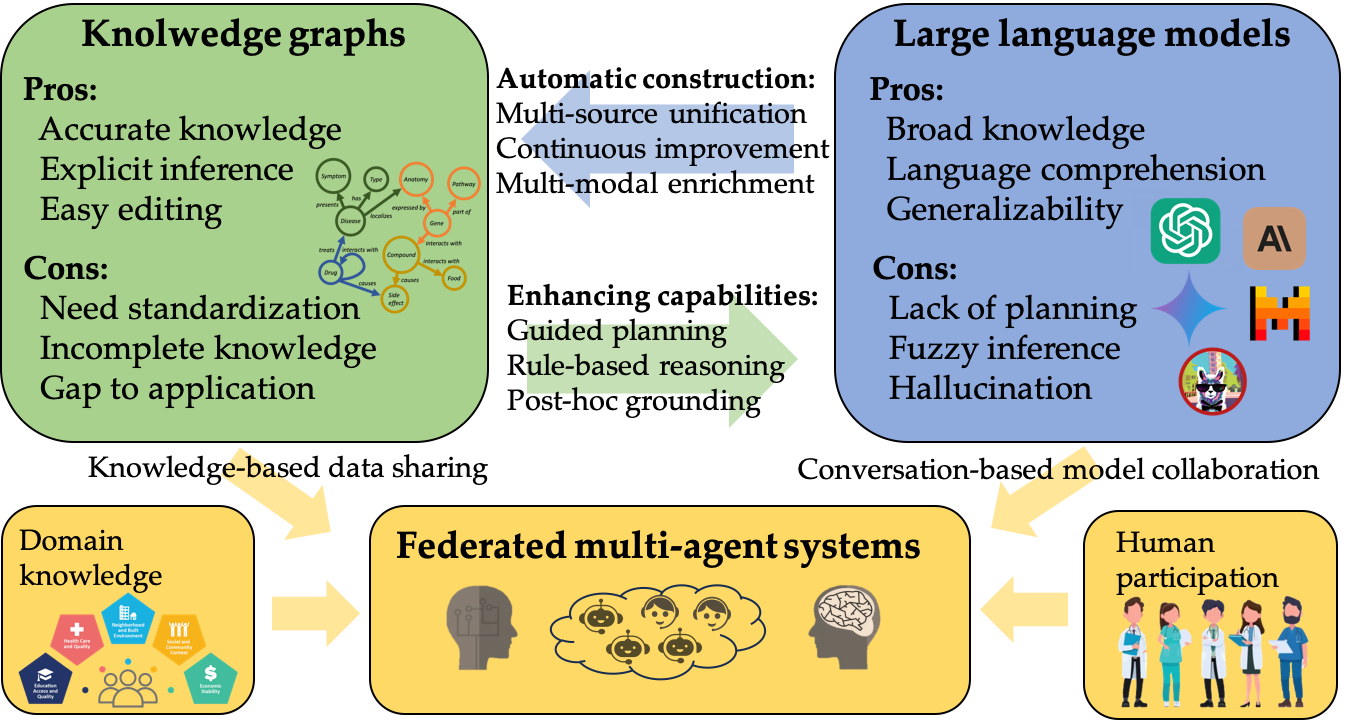
\includegraphics[width=30pc]{submissions/CarlYang2024/figures/intro.png}
\vspace{-3mm}
\caption{Overview of the proposed {knowledge graph and large language model co-learning framework}.}
\vspace{-5mm}
\label{fig:intro}
\end{figure}

%kg+llm existing combinations and limitations
%synergized modeling: roadmap
%KG for LLM: new knowledge, knowledge representation, interpretation-- do not rigorously address the unique challenges in healthcare
%LLM for KG: embedding, completion, construction-- do not comprehensively handle the unique challenges in healthcare
%LLM+KG for health: specific applications without fundamentally improving LLMs and KGs for healthcare
%multi-agent: role play-- do not consider the unique challenges in healthcare regarding privacy, values and disparity
Recently, significant research attention has been drawn to the synergies between KGs and LLMs \cite{pan2023large, pan2024unifying, pan2024integrating, wang2021kepler, yu2022jaket, yasunaga2022deep, jiang2024efficient}, due to their naturally complementary advantages (Figure \ref{fig:intro}). 
The construction and modeling of KGs have often relied on advances in natural language processing (NLP), with recent efforts intensively exploring language models towards the embedding \cite{wang2022language, yu2022cocodr, xie2023lambdakg, choudhary2023complex, zhang2020pretrain, ke2021jointgt}, completion \cite{yao2019kg, kim2020multi, lv2022pre, shen2022joint, choi2023knowledge, wang2021structure, wang2022simkgc, li2023multi, saxena2022sequence, chen2022knowledge, chen2023dipping, lovelace2022framework, xie2022discrimination} and construction \cite{zhu2023llms, ye2022generative, qin2023chatgpt, kommineni2024human, zhang2024extract, vizcarra2024representing, yu2023bear, hu2023llm, meyer2023llm, hofer2024towards, yang2024graphusion, melnyk2021grapher, kumar2020building, chen2022knowprompt, wan2023gpt, wang2024kglink, li2024preliminary, yan2021unified, ding2022prompt, efeoglu2024retrieval, li2022ultra, ayoola2022refined, cattan2021cross, thirukovalluru2021scaling, alt2019improving, guo2021constructing, bosselut2019comet, hao2022bertnet, west2022symbolic} of KGs. 
Studies in the recent years have also bloomed to explore the utilization of KGs for enhancing LLMs through providing new sources of knowledge during pre-training \cite{hu2023survey, wei2021knowledge, yin2022survey, wang2023unifying, sun2022jointlk, liu2021kg, qi2021answering, mavromatis2024gnn, zhang2022greaselm, feng2020scalable, yasunaga2021qa, zhang2019ernie, sun2021ernie, liu2020k, dai2022knowledge, shen2020exploiting, zhang2020bert, tian2020skep, rosset2020knowledge, li2022pre, xiong2020pretrained, he2020bert, su2021cokebert, zhu2023pre, feng2023knowledge, huang2022endowing, agarwal2021knowledge, xu2023kilm, oguz2022unik, tan2024walklm, xu2024bmretriever,sun2020colake, zhang2022dkplm, ye2022ontology, luo2023chatkbqa, martino2023knowledge, chen2020kgpt, santos2022knowledge, moiseev2022skill} or inference \cite{li2023graph, jiang2023unikgqa, luo2024reasoning, sun2024think, wang2024reasoning, luo2023chatrule, wang2023enhancing, besta2024graph, wang2019improving, wang2024knowledge, allemang2024increasing, ji2023rho, feng2023factkb, mcdonald2024reducing, lee2022promptiverse, brate2022improving, wen2023mindmap, wilmot2021memory, logan2019barack, wu2022efficient, guan2024mitigating, dong2024don, sarthi2024raptor, he2024g, han2023pive, edge2024local, gutierrez2024hipporag, liang2024empowering}, and enabling knowledge-based interpretation and evaluation \cite{petroni2019language, jiang2020can, adolphs2021query, shin2020autoprompt, mallen2022not, cohen2023qa, luo2023systematic, liu2023evaluating, orogat2021cbench, zhu2023dyval, bai2024kgquiz, ho2020constructing}. 
Finally, pioneering studies have also been conducted to explore LLM-based multi-agent systems, mostly through prompt-based role-plays to simulate human collaborations \cite{tracy2018agent, tang2024medagents, kaur2024llm, li2024agent, kim2024adaptive, gebreab2024llm, yue2024ct, pan2024agentcoord, xiao2024cellagent}. 

{In this paper, we re-emphasize the promise of KG and LLM co-learning, especially through a structure-oriented retrieval augmented generation (SRAG) paradigm, where LLMs extract structured knowledge from unstructured data, which can be further retrieved to enhance the capabilities and reliabilities of LLMs during applications.}
Specifically, we give examples and discuss several natural and promising use cases where LLMs can be utilized to automate the construction of high-quality KGs. Furthermore, we summarize and highlight several limitations of current LLMs that can be potentially mitigated through the utilization of KGs. Finally, we envision a federated multi-agent system where models and data are disentangled while humans and knowledge are deeply engaged. Future directions are further discussed in the end.
\section{LLM-aided KG Construction}
In this section, we study and establish the advantages of utilizing LLMs for the construction of KGs, by demonstrating their effectiveness in improving the \textit{accuracy}, \textit{consistency}, \textit{coverage}, and \textit{freshness} of knowledge. %Generally speaking, current research and practice on KGs are intensive but mostly around specific types of entities. 
Popular KGs such as Freebase \cite{bollacker2008freebase}, Yago \cite{suchanek2008yago} and Wikidata \cite{vrandevcic2014wikidata} contain hundreds of millions of real-world entities like people, places, and things, along with their multi-typed relations. However, since the KGs are collected and curated by different platforms and institutions, they do not use a unified coding system or thesaurus. The varying terminologies due to different conventions or abbreviations can lead to high degrees of duplication and inconsistency when multiple KGs are directly put together. 
Moreover, the sheer amounts of data in existing KGs are enormous, but the knowledge is still never comprehensive enough to serve various needs of real-world applications, especially those requiring rapidly updated knowledge.
%A few studies have attempted to construct general-purpose healthcare KGs through integrating existing ones \cite{su2023biomedical, cornet2008forty, santos2020clinical}, but they heavily rely on existing coding systems and thesauruses \cite{harrison2021icd, lipscomb2000medical, bodenreider2004unified} for entity alignment across KGs, which often fail in front of varying terminologies such as due to different conventions or abbreviations, leading to high degrees of duplication and inconsistency. 
Recently, pioneering studies including ours have demonstrated strong promise of utilizing LLMs to automate the construction, integration, and enrichment of KGs \cite{zhu2023llms, ye2022generative, qin2023chatgpt, kommineni2024human, zhang2024extract, vizcarra2024representing, yu2023bear, hu2023llm, meyer2023llm, hofer2024towards, yang2024graphusion}. In the following, we give several examples of promising attempts of these kinds and discuss more natural use cases of LLMs and multi-modal foundation models (MMFMs) toward constructing high-quality KGs as promising future directions. 

\subsection{Integrating existing KGs}
% \carl{Need some overviews about motivation, challenge, why LLMs are promising, recent works using LLMs (ours), other recent works, future directions}
%HiPrompt, PromptLink and other LLM-based KG integration
KG integration, also known as knowledge fusion or knowledge alignment, represents a fundamental challenge in the broader landscape of knowledge engineering, which involves integrating multiple KGs that originate from varied sources and formats~\cite{yan2024knownet,lu2022open}.
% The integration of existing KGs presents both great premise and significant challenges in knowledge engineering. 
While individual KGs often excel in specific domains or use cases, their true potential can be unlocked through effective integration, enabling more comprehensive and robust knowledge representation~\cite{himmelstein2017systematic,santos2020clinical}. 
As the number and diversity of KGs continue to grow, the need for effective integration methods becomes increasingly critical.

However, the integration of existing KGs faces several key challenges: (1) \textit{semantic heterogeneity across sources}: Different KGs often use varying terminologies, definitions, and contextual frameworks to represent similar concepts~\cite{liu2022selfkg}; 
(2) \textit{varying granularity levels in knowledge representation}: KGs may differ in the detail and depth with which they describe entities and relationships, impacting the consistency and usability of integrated data. 
Although several neural approaches have been proposed for entity alignment on KGs~\cite{wang2018cross,zhu2020collective,yan2021dynamic}, these methods generally depend heavily on labeled data for training. However, obtaining sufficient labeled data often involves substantial manual effort and can be rather costly.

LLMs have emerged as a promising solution to these challenges with unique advantages: 
First, their strong natural language understanding capabilities enable them to capture semantic relationships among concepts that may be missed by traditional string-matching or embedding-based approaches \cite{chen2023dipping}. 
Second, LLMs can draw on their extensive knowledge acquired during pre-training to aid in disambiguating entities and mapping relationships across different KGs \cite{sancheti2024llm}.
Third, LLMs possess robust few-shot learning abilities, making them particularly valuable for specialized domain applications where labeled data are limited \cite{brown2020language,agrawal2022large}.

\begin{figure}[htbp]
    \begin{center}
    %\framebox[4.0in]{$\;$}
    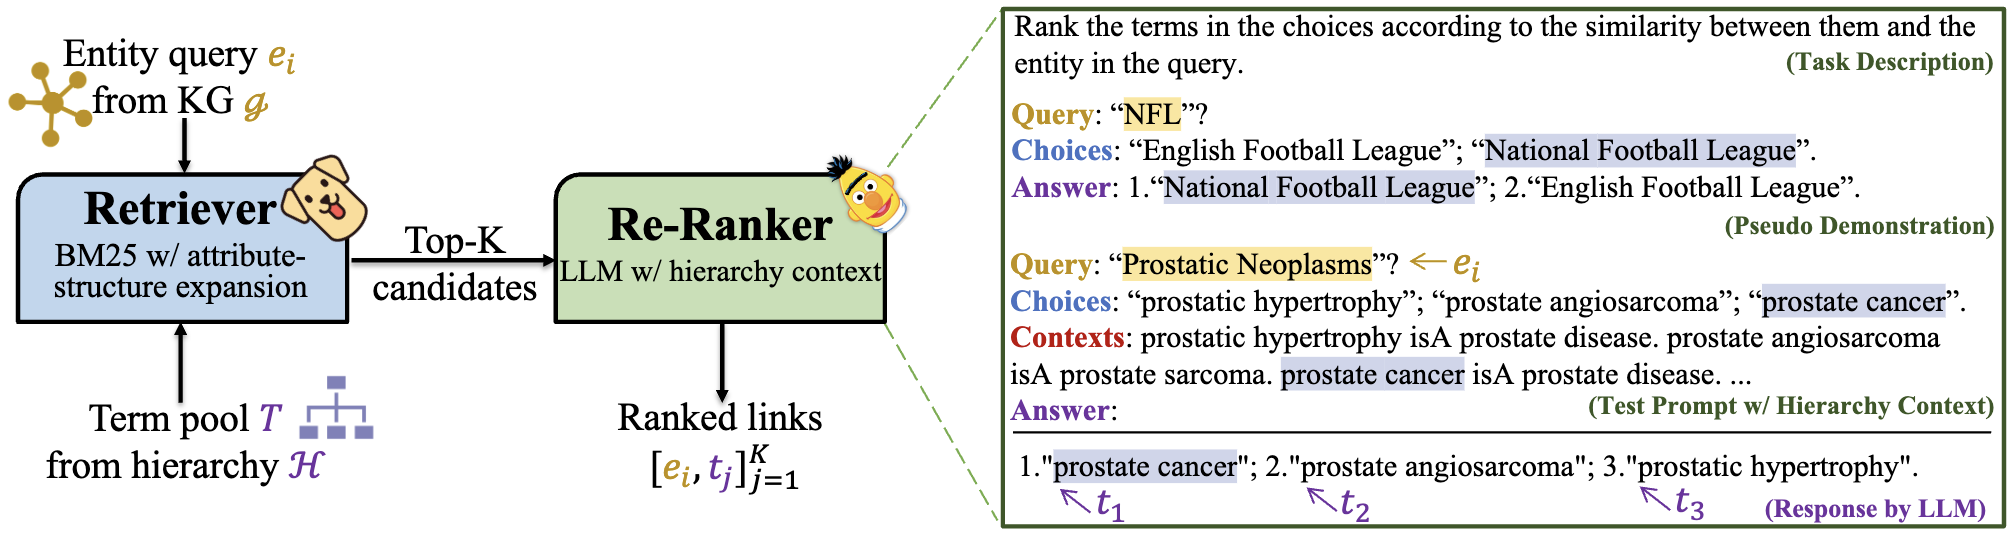
\includegraphics[width=.95\columnwidth]{submissions/CarlYang2024/figures/hiprompt.png}
    \end{center}
    \vspace{-4mm}
    \caption{The overall framework of Hiprompt.}
    \label{fig:hiprompt}
     \vspace{-2mm}
\end{figure}

Recent work has demonstrated the effectiveness of LLM-based approaches in KG integration. 
For example, Lu et al.~\citep{lu2023hiprompt} developed HiPrompt (framework shown in Figure~\ref{fig:hiprompt}), which aligns entities between biomedical KGs and standardized hierarchical entity taxonomies. 
This task poses significant challenges due to the scarcity of available pairs and the inconsistent naming conventions between KGs and entity taxonomies.
Their two-stage approach combines traditional information retrieval techniques (BM25) with LLM-based re-ranking using hierarchy-oriented prompts, achieving superior performance in few-shot biomedical knowledge-graph integration.  
Building on this direction, Xie et al.~\citep{xie2024promptlink} developed PromptLink, a framework that leverages both domain-specific language models and GPT-4 for cross-source biomedical concept linking. The framework employs a two-stage prompting mechanism by first eliciting the biomedical prior knowledge from the LLM for the concept linking task and then enforcing the LLM to reflect on its own predictions to further enhance their reliability. 
PromptLink’s success in zero-shot scenarios illustrates the potential of LLMs to generalize across diverse data sources without extensive training data.

In contrast to the two LLM approaches that primarily use LLMs for ranking candidate sets, AutoAlign \cite{zhang2023autoalign} employs off-the-shelf LLMs to construct a predicate-proximity graph that captures relationships between entity types rather than individual entities. It then aligns the entity embeddings of two KGs into a common vector space by calculating similarity based on entity attributes.


These advances suggest several promising future directions for LLM-aided KG integration. For example, LLMs could potentially facilitate the continuous integration of new knowledge into existing KGs dynamically and automatically by identifying and resolving conflicts between new and existing information, while maintaining consistency across the integrated knowledge base. Such real-time data integration is especially beneficial for dynamic applications like live event monitoring and real-world decision-making. {Furthermore, integrating KGs with LLMs remains challenging due to the risk of generating false or untrustworthy information~\cite{yang2024give}. To mitigate this issue, there is a growing need for improved human-in-the-loop systems. Specifically, enhanced interfaces~\cite{hassan2017claimbuster,nakov2021automated} can enable experts to more effectively verify and interpret LLM-generated recommendations, ensuring greater reliability and transparency.}



% Lu et al.~\citep{lu2023hiprompt} propose HiPrompt, an innovative framework that leverages LLMs for biomedical knowledge fusion. Their work addresses the challenge of aligning entities from biomedical KGs with terms in a standardized hierarchical index system, a task that traditionally suffers from scarce labeled data and inconsistent naming conventions. HiPrompt employs a two-stage approach: a retrieval module using BM25 with expanded entity and term representations, followed by an LLM-based re-ranking module that utilizes hierarchy-oriented prompts. This approach enables effective few-shot learning, outperforming both conventional unsupervised methods and neural embedding models in zero-shot and one-shot settings. It demonstrates the potential of LLMs in capturing complex semantic relationships and hierarchical constraints in KG integration tasks, even with minimal supervision. Their findings suggest that LLM-aided approaches could significantly advance the field of KG construction and integration, particularly in domains with limited labeled data.

% Another notable example is PromptLink~\citep{xie2024promptlink}, which leverages LLMs for cross-source biomedical concept linking. PromptLink combines the strengths of biomedical-specialized pre-trained language models and GPT-4 to address the challenges of inconsistent naming conventions across different data sources. The framework employs a two-stage prompting mechanism that efficiently filters candidates and generates reliable linking predictions, including NIL predictions when no suitable match is found. By outperforming conventional string-matching and machine learning-based methods in zero-shot accuracy, PromptLink demonstrates the potential of LLMs in enhancing KG integration tasks. This approach is particularly valuable in domains where labeled data is scarce and the ability to generalize across various data sources is crucial.

\subsection{Constructing and Completing KGs}
KGs have high-standard requirements on the quality of knowledge, regarding accuracy, consistency, coverage and freshness. No matter constructed through manual curation, NLP tools, or their combinations, KGs can unavoidably include erroneous knowledge. Moreover, when multiple KGs are integrated, conflicting knowledge can emerge. Finally, new knowledge is constantly generated from new experiments and research, making existing knowledge inaccurate and incomplete. LLMs have emerged as a promising solution, leveraging the vast and adaptable knowledge acquired during pre-training to overcome these limitations \cite{petroni2019language, yu2024kola, xu2024clingen, alkhamissi2022review}. 
The key advantage of LLMs for KG construction and completion is their ability to generate novel, semantically coherent information with minimal reliance on additional labeled data.

% The key advantage of LLMs in this domain lies in their ability to generate novel, semantically coherent information that can supplement and enrich existing KGs. Unlike rule-based or supervised machine learning approaches, LLMs can leverage their extensive understanding of language and the world to infer missing connections, identify new entities, and uncover implicit relationships - all without being constrained by the limitations of manually curated training data.

Recent studies have highlighted the effectiveness of LLM-based approaches for KG construction and completion. Zhu et al. \citep{zhu2023llms} utilize in-context learning capabilities of LLMs to complete tuples with missing entities or relations to generate new knowledge triplets for augmenting existing KGs.
Wei et al. \citep{wei-etal-2023-kicgpt} and Wang et al. \citep{wang-etal-2024-kc} tackle KG completion as a candidate identification and ranking task, proposing a “retrieve-rank” pipeline where LLMs are used to rerank top-retrieved entities, thus creating additional knowledge triplets.

An alternative approach to prompting LLMs involves using code-based prompts,  rather than natural language, to incorporate new entities into existing KGs~\cite{bi2024codekgc,zeng2024codetaxo}. 
Code LLMs, extensively trained on structured data such as programming code, are inherently well-suited to the structured nature of KGs.
Using a code-based interface enables more effective handling of graph-like structures, logical relationships, and precise reasoning~\cite{madaan2022language,chen2023program,shi2024agent}.
Specifically, Bi et al. \cite{bi2024codekgc} first encoded the schema of KGs by modeling code definitions, to capture the structural information inherent in the data. They then employed chain-of-thought prompting to produce accurate knowledge triples. This methodology demonstrates improved performance over traditional natural language-based prompts. 
Similarly, Zeng et al.~\citep{zeng2024codetaxo} proposed CodeTaxo, which represents entities within a base 'Entity' class, mirroring hierarchical relationships in programming constructs. This approach enables LLMs to efficiently create taxonomic structures by leveraging syntactic capabilities commonly used in code tasks, thus enhancing the organization and completeness of KGs. 
% Another notable example is CodeTaxo~\citep{zeng2024codetaxo} which encapsulates entities in a base class 'Entity' to better characterize hierarchical relations similar to programming constructs. This enables the LLM to efficiently process and generate taxonomic structures by leveraging its strong syntactic capabilities, which are typically associated with code understanding tasks. By combining the LLM's natural language understanding with its code-related skills, CodeTaxo demonstrates the versatility of these models in enhancing the completeness and organization of KGs.


The above methods primarily focus on prompting LLMs for KG construction and completion. While these methods show promise, they fall short in fully adapting LLMs to target tasks and can suffer from hallucination issues. To address these limitations, several studies aim to improve the quality of LLM-generated content for KG tasks. 
{Zhang et al. \cite{zhang2024extract} presented a three-phase framework for constructing KGs with LLMs to enhance contextual understanding and schema alignment. 
It starts with open information extraction to identify relation triplets from unlabeled textual corpora, followed by schema definition where LLMs generate contextually relevant descriptions for schema components. 
Finally, the extracted triplets are aligned with the schema.  
To further enhance the quality of the extracted
triplets and minimize the risk of misinformation, a schema retriever is used to generate a list of candidate entities and relations to guide the triplet extraction steps. This approach works for both predefined schemas and situations where the schema needs to be inferred from the context.
}
% \cite{zhang2024extract} presents a three-phase framework for constructing KGs with LLMs to enhance contextual understanding and schema alignment. The process begins with open information extraction, where relational triplets are identified from unlabeled textual corpora. Next, LLMs is used to define schema components by generating contextually relevant, human-like descriptions. In the final canonicalization phase, extracted triplets are aligned with the schema to ensure consistency and reduce redundancy. This adaptable framework is effective in both predefined schema settings and scenarios where schema must be inferred from context.
Additionally, various studies explored fine-tuning LLMs specifically for KG completion. Zhang et al.~\cite{kopa} proposed KOPA that first applies structural pre-training to create embeddings of entities and relations in KGs, and project embeddings into the textual space as virtual knowledge tokens. These tokens act as prefixes in LLM input prompts, enabling structure-aware reasoning that leverages both the generative power of LLMs and the retrieval of structured KG information to improve the accuracy and completeness of KG completion tasks. 
Jiang et al.~\citep{jiang2024kg} introduced KG-FIT for using open-world knowledge from LLMs to enhance KG embeddings. It initially constructs a semantically coherent, hierarchical structure of entity clusters, guided by LLM-powered entity representations. It then fine-tunes these embeddings by integrating the hierarchical structure with textual embeddings. This hybrid approach allows KG-FIT to capture both the semantic depth of LLMs and the structural information intrinsic to KGs, resulting in more comprehensive KG representations.



% TaxoPrompt~\citep{xu2022taxoprompt}, a prompt-based method for self-supervised taxonomy expansion that effectively leverages the global structure of taxonomies. TaxoPrompt integrates the taxonomic context into the training of a language model (LM) by employing a customized random walk algorithm that captures relational paths within the taxonomy. This context is then used in a prompt-tuning framework to transform the taxonomy expansion problem into a hypernym generation task. During the process, a template creates a cloze task where the LM predicts missing hypernyms based on provided context, thus maintaining the structural integrity of the taxonomy.


% https://arxiv.org/abs/2405.16412
% https://dl.acm.org/doi/pdf/10.1145/3637528.3671469
% https://arxiv.org/pdf/2408.09070
% https://www.ijcai.org/proceedings/2022/0615.pdf

\begin{figure}[htbp]
    \begin{center}
    %\framebox[4.0in]{$\;$}
    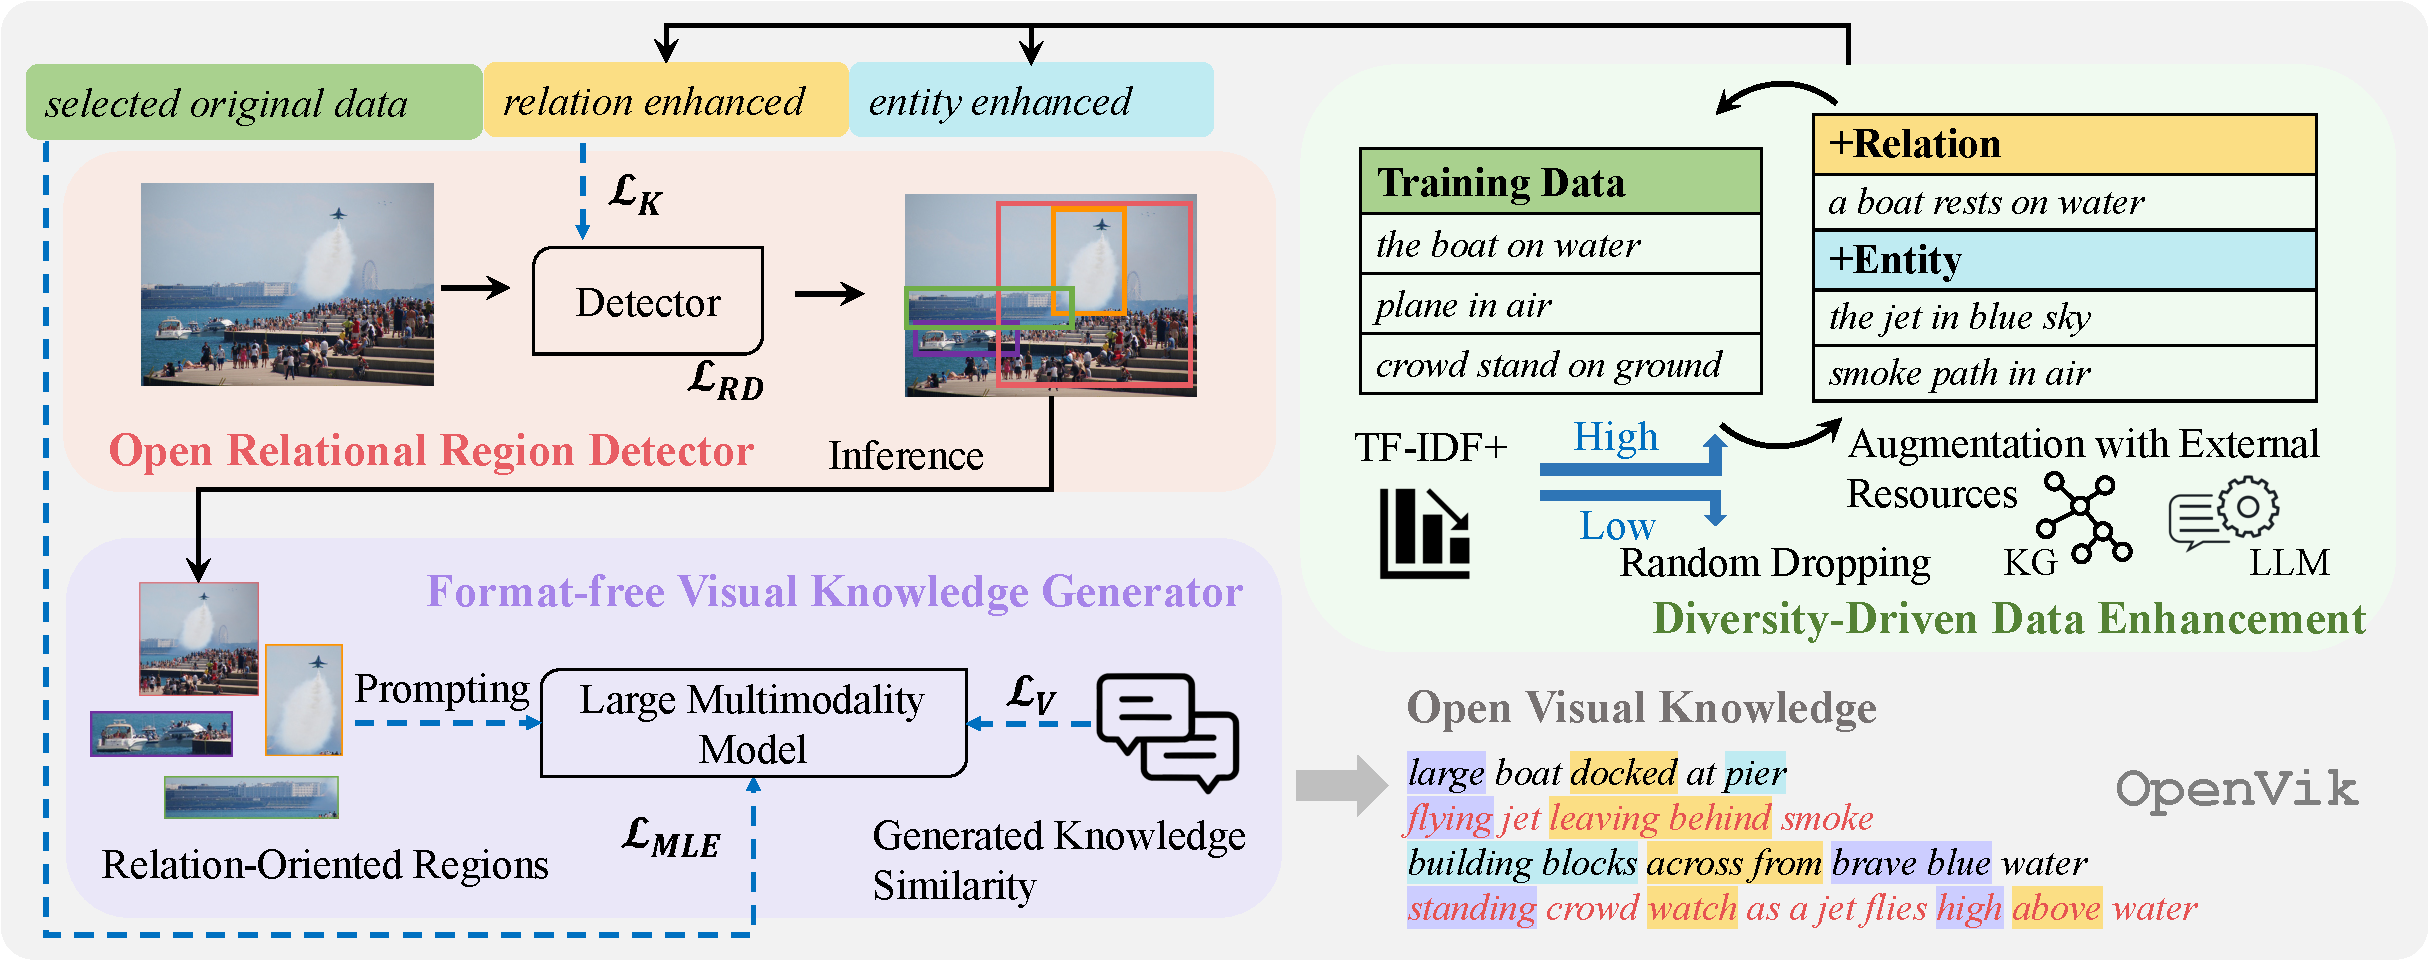
\includegraphics[width=.95\columnwidth]{submissions/CarlYang2024/figures/openvik.pdf}
    \end{center}
    % \vspace{-3mm}
    \caption{{The overall framework of OpenVik consists of two main components: (1) an open relational region detector, highlighted in the orange and purple panels, which includes a region regression loss ($\mathcal{L}_{\text{RD}}$) and a regional description loss ($\mathcal{L}_{\text{K}}$), and (2) a format-free visual knowledge generator, incorporating knowledge generation loss ($\mathcal{L}_{\text{MLE}}$) and diversity regularization ($\mathcal{L}_{\text{V}}$). These modules work collaboratively to extract open visual knowledge, incorporating novel entities and diverse relations in a format-free manner.}}
    \label{fig:openvik}
    % \vspace{-5mm}
\end{figure}



\subsection{Enriching KGs with multi-modality data}
Traditionally, specialized models and algorithms have been developed to process and analyze various modalities of data such as tables, texts, images, and time series. These methods can hardly perform integrative analysis across data modalities and generalize across different data platforms. Recently, LLM-based multi-modality foundation models (MMFMs) have shown strong promise in analyzing multi-modality data through the unified interface of languages \cite{yang2023dawn, fei2022towards, li2024multimodal, li2024llava, zhang2023biomedgpt}.
Integrating multi-modal data into KGs creates a more comprehensive representation of entities and their relationships, enhancing performance in open-world applications like image classification and visual question answering \cite{chen2024knowledge}. Many studies focus on using MMFMs for specific tasks, such as entity extraction \cite{sun2024umie,li2023prompting,hu2023prompt}, relation extraction \cite{yu2023visually,li2024zero,li2024pixels}, or event extraction \cite{chen2024schema,rasheed2024glamm}. However, these works often isolate extraction tasks without unifying entities and relations into a structured KG.
{A pioneering approach in this direction is OpenVik \cite{cui2024open} (framework shown in Figure~\ref{fig:openvik}). It first trains an open relational region detector to locate image regions containing relational information. 
It then employs a visual knowledge generator to create format-free knowledge descriptions by prompting a large visual language model. Through the use of MMFM, OpenVik advances KG completion by integrating rich visual context, expanding knowledge coverage, and enhancing the accuracy of representation within the resulting KG.}
Application-wise, Yang et al.~\cite{yang2024hierarchical}  proposed an automated approach to constructing product KGs from raw images in e-commerce. This method first employs vision-language models (VLMs) to extract detailed image information and then uses an LLM to reason and infer additional KG properties not visually present, hierarchically expanding, and linking nodes to develop comprehensive, scalable KGs without human input.


% https://www.cs.emory.edu/~jyang71/files/openvik.pdf
\newcommand{\gG}{\mathcal{G}\xspace}
\newcommand{\gL}{\mathcal{L}\xspace}
\newcommand{\gZ}{\mathcal{Z}\xspace}

\section{KG-guided LLM Enhancement}
LLMs have shown impressive communication and question-answering capabilities, demonstrating strong promise in various applications \cite{wang2024survey, wu2023bloomberggpt, cui2023chatlaw, chen2023genept, singhal2023large, singhal2023towards, haupt2023ai, nori2023capabilities, lee2023benefits, fleming2023assessing, chen2023meditron, yang2022large, luo2022biogpt, agrawal2022large, mehandru2024evaluating, zhang2023biomedgpt, biswas2023role, dash2023evaluation}. 
%answering medical questions \cite{singhal2023large, singhal2023towards, haupt2023ai, nori2023capabilities, lee2023benefits, fleming2023assessing, chen2023meditron}, extracting clinical information \cite{yang2022large, luo2022biogpt, agrawal2022large} and assisting clinical decisions \cite{mehandru2024evaluating, zhang2023biomedgpt, biswas2023role, dash2023evaluation}. 
%However, LLMs are also shown to ``hallucinate'' false outputs and unsubstantiated answers \cite{hal, hal3, hal4}, preventing their adoption in diverse fields, especially those with high-standard requirements on the accuracy and factuality of responses such as healthcare \cite{hal7}. Recently, many technical frameworks have been proposed to detect or avoid hallucinations in LLMs, such as based on supervision for reinforcement learning \cite{hal8}, statistical uncertainty measurements \cite{hal} and \todo{xxx \cite{}}. 
However, to reliably model domain-specific data and generate factual and accurate answers, LLMs still face the challenges of lacking domain knowledge, fuzzy inferences, and hallucination \cite{hu2023large, mousavi2024your, yadkori2024believe, asai2024selfrag,yu2024rankrag, liu2023evaluating, zhu2023dyval, zhuo2024roles, yuan2024back, wang2023boosting, ji2023survey, bai2024hallucination, tonmoy2024comprehensive, maynez2020faithfulness, xiao2021hallucination, farquhar2024detecting, ji2023towards, chen2024inside}.
% \textit{lack of knowledge} \cite{hu2023large, mousavi2024your, xu2024kg, becker2024cycles, yadkori2024believe, kim2024m}, \textit{fuzzy inference} \cite{liu2023evaluating, zhu2023dyval, bai2024kgquiz, zhuo2024roles, baek2024researchagent, yuan2024back, wang2023boosting}, and \textit{hallucination} \cite{ji2023survey, bai2024hallucination, tonmoy2024comprehensive, maynez2020faithfulness, xiao2021hallucination, farquhar2024detecting, ji2023towards, chen2024inside}
Retrieval augmented generation (RAG) \cite{lewis2020retrieval}, which aims at retrieving query-relevant evidence and generating evidence-based answers, has strong promise in evidence-critical domains. However, effective and efficient RAG for complex queries is still challenging which requires LLMs to be able to (1) generate logical plans for retrieving multiple pieces of relevant evidence from complex data, (2) conduct valid reasoning and inference to compose the pieces of evidence towards generating coherent answers, and (3) reliably guarantee the detection and removal of errors. In the following, we discuss how these challenges can be addressed with well-designed planning, reasoning, and reflection frameworks with the help of KGs.

{
\newcommand{\ourmethod}{\texttt{RoG}\xspace}
\subsection{Planning with domain knowledge}
% \carl{Linhao, the current 3.1 is too long-- we aim to write about 12 pages of main contents in total and the plan is to write about 2 (front page/intro)+ 3 (sec 2) + 3 (sec 3) + 2 (sec 4) + 1 (sec 5) + unlimited references. Can you perhaps try to separate the current contents into 3.1 (planning) and 3.2 (reasoning)? Please try to re-organize/re-write the contents more so they also read differently from your RoG paper. Please also add some discussions about more related recent works separately in both subsections. I added a reference in 3.3, but please let me know if you are not sure about what to write in 3.3. Thanks!}\\
While LLMs excel in many NLP tasks \cite{brown2020language,bang2023multitask}, they still face challenges in acquiring domain knowledge. To address this issue, many attempts seek assistance from KGs, which are often constructed to represent knowledge in specific domains, such as medicine \cite{bodenreider2004unified}, law \cite{kang2024bridging}, and finance \cite{liu2019anticipating}. The integration of KGs and LLMs has shown promising results in various applications, such as question answering \cite{jiang2023unikgqa}, recommendation \cite{wang2023enhancing}, and dialogue systems \cite{tuan2022towards}. Despite the success, there are still challenges in effectively obtaining useful information from KGs and incorporating them into LLMs. 

Existing methods typically depend on a retriever to obtain relevant triples. For example, Baek et al. \cite{baek2023direct} proposed a direct retrieval method to retrieve relevant triples from KGs. However, the retriever may not always retrieve the most relevant triples, leading to suboptimal performance. Additionally, KGs contain a wealth of domain-specific knowledge, making it challenging for LLMs with limited domain expertise to comprehend and utilize this information. To further unleash LLMs' capabilities of leveraging domain knowledge, the \textit{plan-and-solve} paradigm \cite{wang2023plan} has been proposed, in which LLMs are prompted to first generate a plan. Based on the plan, LLMs can retrieve the relevant domain knowledge and conduct reasoning to generate answers \cite{yaoreact}. However, existing methods are incapable of handling the complex structured knowledge in KGs to enable effective planning and reasoning. To address this issue, we propose a \textit{planning-retrieval-reasoning} framework named \ourmethod that enables LLMs to plan and reason on KGs \cite{luo2024reasoning}. The overall framework is illustrated in \Cref{fig:rog}.

\begin{figure}[htbp]
    \begin{center}
    %\framebox[4.0in]{$\;$}
    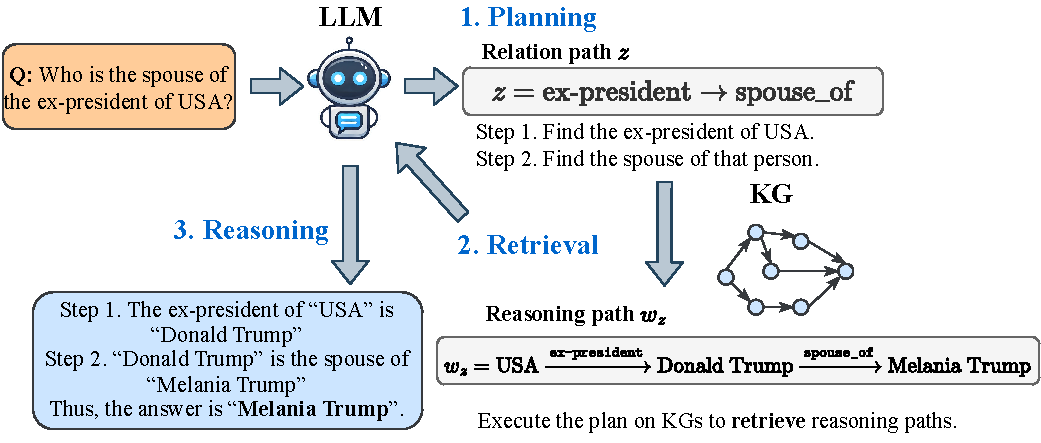
\includegraphics[width=.85\columnwidth]{submissions/CarlYang2024/figures/rog.pdf}
    \end{center}
    % \vspace{-3mm}
    \caption{The overall framework of planning and reasoning on KGs (\ourmethod).}
    \label{fig:rog}
    % \vspace{-5mm}
\end{figure}

\ourmethod first generates several relation paths that are grounded by KGs as plans. Relation paths, which capture semantic relations between entities, have been utilized in many reasoning tasks on KGs \cite{wang2021relational,xusubgraph}. Based on relation paths, we can always retrieve the latest knowledge from KGs with a simple constrained breadth-first search. Therefore, relation paths can serve as faithful plans to guide the retrieval and reasoning on domain-specific KGs. Additionally, by treating relation paths as plans, we can make sure the plans are grounded by KGs, which enables LLMs to retrieve relevant knowledge and conduct faithful reasoning. To this end, we formulate our \ourmethod as an optimization problem that aims to maximize the probability of reasoning the answer from a KG $\gG$ w.r.t the question $q$ by generating relation paths $z$ as the plan:
\begin{equation}
    % \setlength\abovedisplayskip{1pt}%shrink space
    % \setlength\belowdisplayskip{1pt}
    \label{eq:plan}
    P_\theta(a|q,\gG) = \sum_{z\in\gZ}P_\theta(a|q,z,\gG)P_\theta(z|q),
\end{equation}
where $\theta$ denotes the parameters of LLMs {and $a$ denotes the final answer.} To enable accurate planning with domain knowledge, we design two instruction tuning tasks: 1) \textit{planning optimization}, which distills the knowledge from KGs into LLMs to generate faithful relation paths as plans; 2) \textit{retrieval-reasoning optimization}, which enables LLMs to reason based on the retrieved reasoning paths.
{
The final objective function of \ourmethod is the combination of the planning optimization and retrieval-reasoning optimization, which can be formulated as
\begin{equation}
    \setlength\abovedisplayskip{1pt}%shrink space
    \setlength\belowdisplayskip{1pt}
    \label{eq:final_obj}
    \gL = \log \underbrace{P_\theta(a|q,\gZ^*_K,\gG)}_{\text{Retrieval-reasoning}} + \underbrace{\frac{1}{|\gZ^*|}\sum_{z\in Z^*}\log P_\theta(z|q)}_{\text{Planning}},
\end{equation}
where we use the shortest paths $\gZ^*\subseteq\mathcal{Z}$ between $q$ and $a$ in KGs as supervision signals. We maximize the probability of LLMs generating faithful relation paths through distilling the knowledge from KGs.
}
In this way, with the proposed \ourmethod, LLMs can effectively retrieve domain knowledge from KGs with planning, which significantly enhances the reasoning capability of LLMs.
}

{
    \newcommand{\ourmethod}{\texttt{GCR}\xspace}
\subsection{Reasoning with structured knowledge}
% https://arxiv.org/abs/2410.13080
KGs capture abundant factual knowledge in a structured format, which provides a faithful knowledge source for improving the reasoning abilities of LLMs \cite{pan2024unifying}. Nevertheless, because of the unstructured nature of LLMs, directly applying them to reason on structured KGs is challenging. Early works focus on fine-tuning LLMs together with structured knowledge from KGs to enrich the knowledge of LLMs for better reasoning \cite{zhang2019ernie,rosset2020knowledge}. For example, KEPLER~\cite{wang2021kepler} directly employs both KG embedding training objective and Masked token pre-training objective into a shared transformer-based encoder. Through fine-tuning, LLMs can better understand the structured knowledge in KGs for reasoning. However, the fine-tuning process is computationally expensive and incapable of efficiently adapting to the evolving real-world knowledge. 

Recently, researchers have combined the strengths of retrieval-based methods with the prompting technique to enable LLMs to reason on KGs \cite{lewis2020retrieval,jiang2023unikgqa}. CoK \cite{wang2023boosting} and KD-CoT \cite{wang2023knowledge} retrieve facts from an external KG to guide the CoT performed by LLMs. To capture graph structure, GNN-RAG \cite{mavromatis2024gnn} adopts a lightweight graph neural network to effectively retrieve knowledge from KGs, which are formatted as a sentence path to elicit the reasoning process of LLMs. Mindmap \cite{wen2023mindmap} builds a prompt-based method that endows LLMs with the capability of comprehending KG and reasoning with it. Despite the success of these methods, they still face challenges in designing principled prompts to represent KGs and conduct reasoning. Moreover, LLMs still have limited capabilities in understanding the graph structure and reasoning with the text-based graph prompts \cite{huang2024can}. 

Different from existing efforts that require a computationally expensive fine-tuning phase or design ad-hot prompts for LLMs,  we recently introduced a KG-constrained reasoning (\ourmethod) paradigm \cite{luo2024graph}. \ourmethod connects unstructured reasoning in LLMs with structured knowledge in KGs, seeking to achieve efficient and effective reasoning on structured knowledge. The overall framework is illustrated in \Cref{fig:gcr}.

\begin{figure}[htbp]
    \begin{center}
    %\framebox[4.0in]{$\;$}
    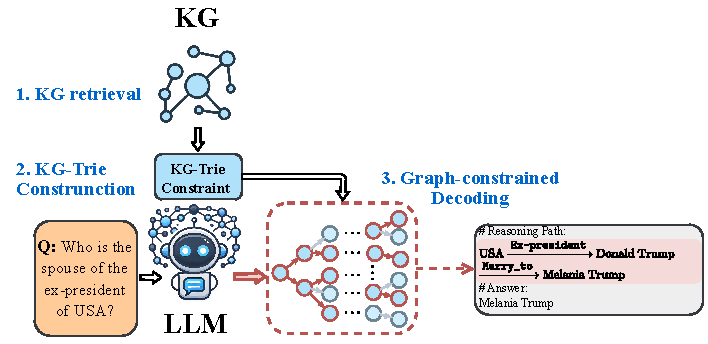
\includegraphics[width=.75\columnwidth]{submissions/CarlYang2024/figures/gcr.pdf}
    \end{center}
    % \vspace{-3mm}
    \caption{The overall framework of KG-constrained reasoning (\ourmethod).}
    \label{fig:gcr}
    % \vspace{-5mm}
\end{figure}

Graph-constrained reasoning, inspired by the concept that LLMs reason through decoding \citep{wei2022chain}, incorporates the KG structure into the LLM decoding process. This enables LLMs to directly reason on graphs by generating reliable reasoning paths grounded in KGs that lead to correct answers. Specifically, given a question, we first adopt a retrieval module to find a relevant KG that is helpful for reasoning. Then, we convert the KG into a structured index, KG-Trie, to facilitate efficient reasoning on KG using LLMs. Trie is also known as the prefix tree \citep{fredkin1960trie} that compresses a set of strings, which can be used to restrict LLM output tokens to those starting with valid prefixes. KG-Trie encodes the reasoning paths in KGs as formatted strings to constrain the decoding process of LLMs. Then, we propose graph-constrained decoding that employs a lightweight KG-specialized LLM to generate multiple KG-grounded reasoning paths and answers. With the constraints from KG-Trie, we ensure faithful reasoning while leveraging the strong reasoning capabilities of LLMs to efficiently explore paths on KGs in constant time. In this way, \ourmethod bridges the gap between structured knowledge in KGs and unstructured reasoning in LLMs, allowing for efficient reasoning on KGs via LLM decoding.

}
\subsection{Reflecting with atomic knowledge}
% \carl{https://arxiv.org/abs/2311.13314}\\
% https://arxiv.org/pdf/2310.11638\\
% https://arxiv.org/pdf/2402.11199\\
LLMs have shown impressive capabilities in encapsulating massive knowledge and conducting reasoning. However, they still face challenges in generating factually correct and faithful responses, especially in the presence of hallucinations \cite{huang2023survey}. KGs store atomic knowledge in a structured format, which can be used to verify the correctness of generated responses and detect hallucinations \cite{agrawal2023can}. To incorporate the factual knowledge from KGs into LLM hallucination detection, Guan et al. \cite{guan2024mitigating} proposed a retrieval-based method called KG-based retrofitting (KGR). KGR retrieves relevant facts from KGs during the LLM reasoning process, which are used to mitigate factual hallucination by retrofitting the initial responses. KGR enables an autonomous knowledge verifying and refining procedure with the factual knowledge retrieved from KGs, which significantly improves the reliability of LLMs. 

The hallucination of LLMs is usually attributed to the lack of factual knowledge of LLMs. To systematically evaluate the factual knowledge inside LLMs, as shown in \Cref{fig:reflecting}a, we propose a novel framework to automatically assess the factual knowledge in LLMs by using KGs \cite{luo2023systematic}. Unlike conventional methods that rely on human-annotated question-answering datasets, we systematically generate valid and diverse questions from KGs
with different difficulties while also ensuring knowledge coverage. Specifically, we retire the atomic knowledge from KGs as sets of triples. Then, we utilize different question generation methods, e.g., template-based and LLM-based methods, to convert the triples into question-answer pairs. The generated pairs are used to evaluate the factual knowledge of LLMs by comparing the generated answers with the ground-truth answers. The evaluation results can be used to reflect the factual knowledge of LLMs. In this way, we can systematically evaluate the factual knowledge of LLMs and provide insights into the hallucination behavior of LLMs, which can be used to improve the reliability of LLMs in various applications. 

Apart from the factual knowledge, the structure of KGs can be also utilized to justify the reasoning process of LLMs. Minh-Vuong et al \cite{nguyen-etal-2024-direct} designed a framework that delves deeper into the CoT reasoning capabilities of LLMs in multi-hop question answering by utilizing KGs, as shown in \Cref{fig:reflecting}b. The framework contains two evaluation modules: discriminative evaluation and generative evaluation. The discriminative evaluation aims to analyze whether the LLMs possess enough knowledge to conduct faithful reasoning. It feeds both valid and invalid reasoning paths retrieved from KGs into LLMs and asks them to predict the validity of these paths. The generative evaluation, on the other hand, aims to evaluate the faithfulness of the reasoning process of LLMs by grounding it on KGs. Given a reasoning process generated by LLMs, the generative evaluation module retrieves the facts from KGs, which are compared with the ground-truth reasoning paths. The evaluation results can be used to reflect the reasoning capabilities of LLMs and provide insights into the faithfulness of LLM reasoning. Based on the findings, although LLMs have shown impressive reasoning capabilities, they still face challenges in conducting faithful reasoning, especially in multi-hop question answering. 

\begin{figure}[htbp]
    \begin{center}
    %\framebox[4.0in]{$\;$}
    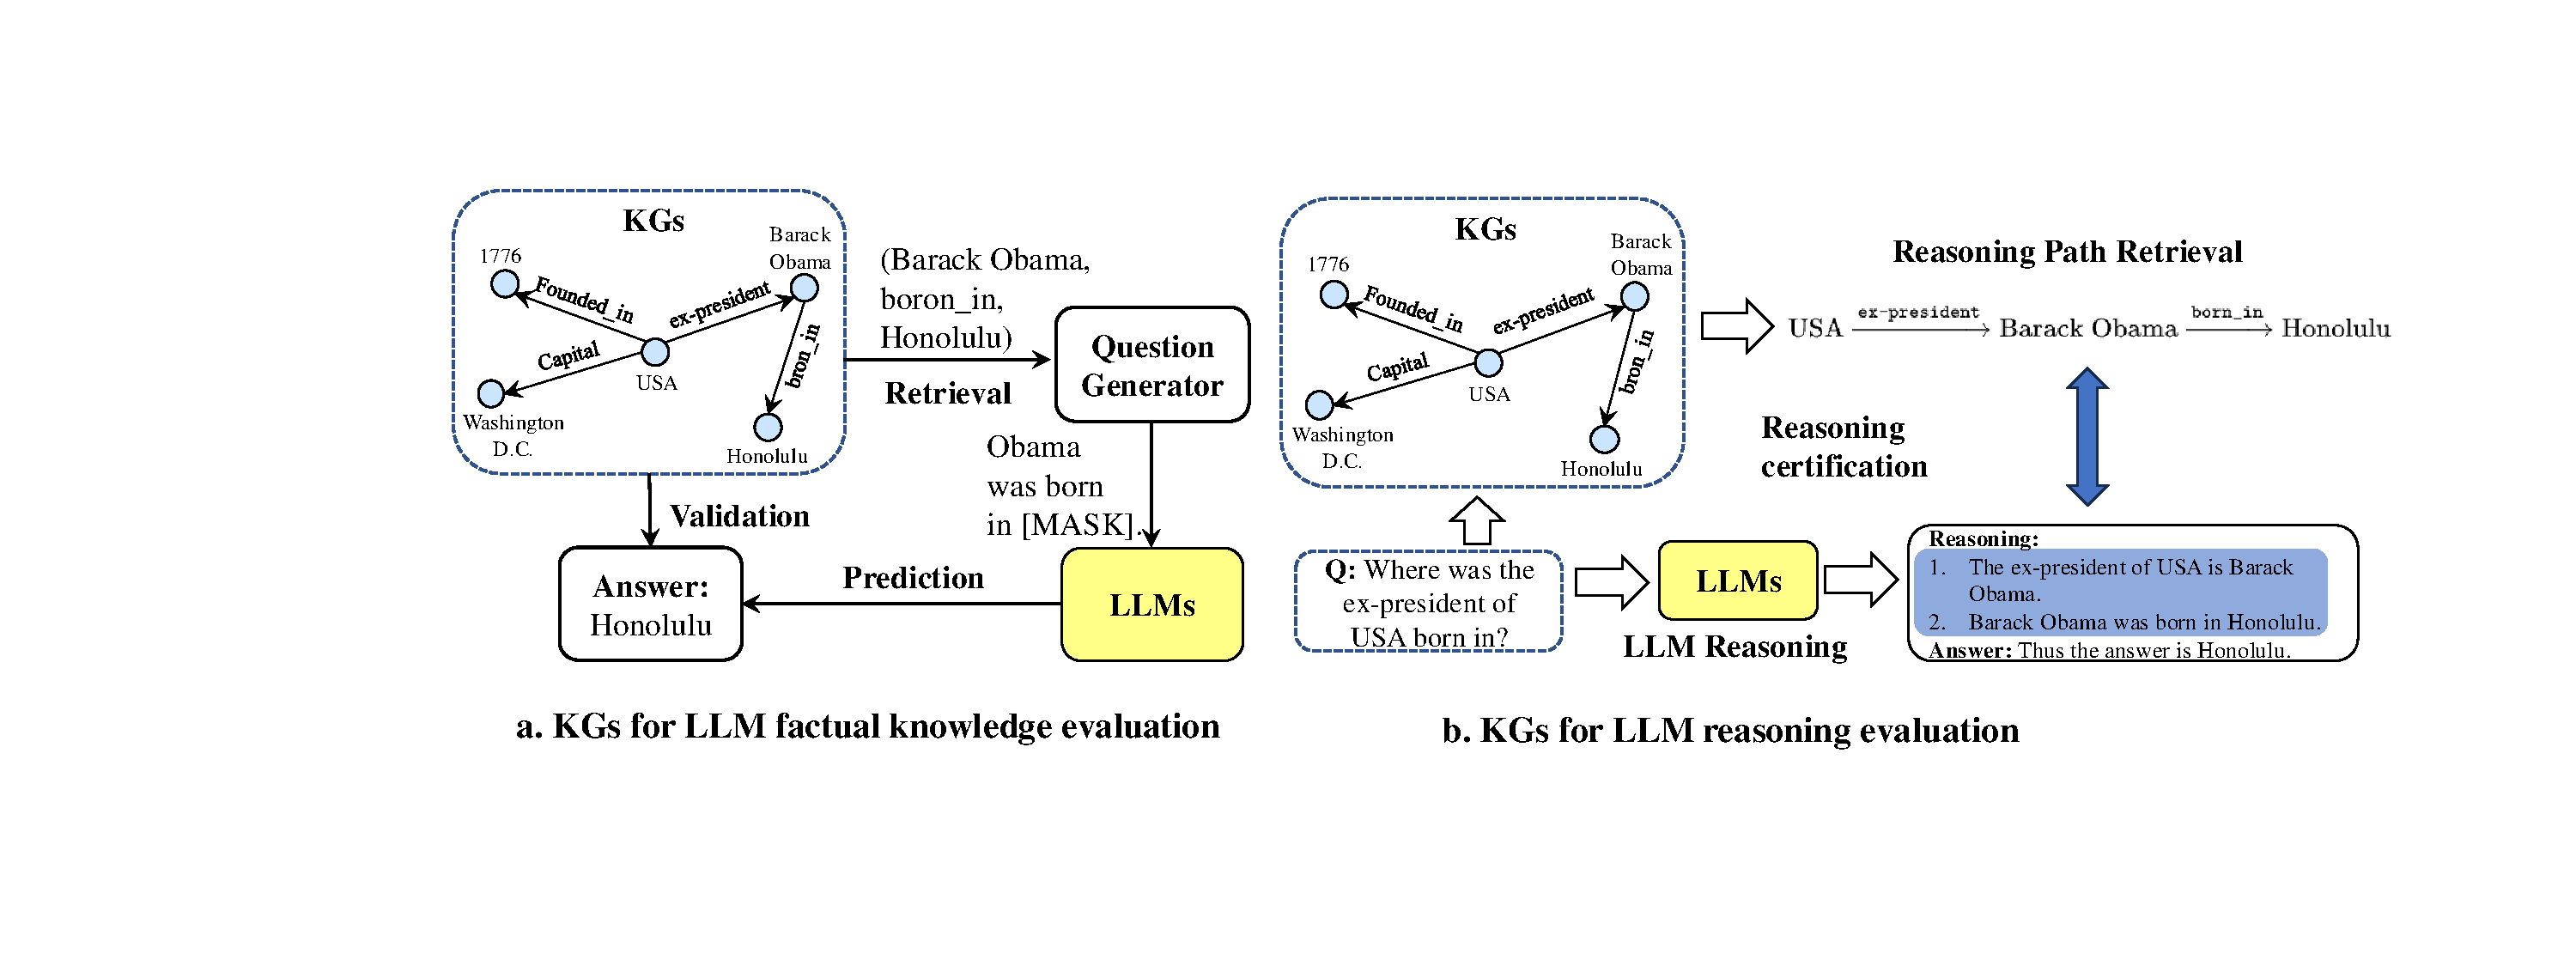
\includegraphics[width=1\columnwidth]{submissions/CarlYang2024/figures/reflecting.pdf}
    \end{center}
    % \vspace{-3mm}
    \caption{The illustration of LLM reflection with KGs. (a) The evaluation of the factual knowledge inside LLMs. (b) The evaluation of the reaosning process of LLMs with KGs.}
    \label{fig:reflecting}
    % \vspace{-5mm}
\end{figure}
\section{Knowledge-aware Multi-agent Federation}
%\carl{TODO: will work on this section over the weekend}\\
While KGs and LLMs can mutually enhance each other, data are properties and many real-world datasets are privately collected and owned by different institutions, which cannot be simply put together to train more powerful models. 
Moreover, many real-world applications require domain-specific knowledge that may not have been captured by general-purpose KGs and LLMs yet, and such knowledge can also be private properties. 
Finally, while the development of KGs and LLMs is highly automated and data-driven, the values and needs of different human stakeholders may not have been properly reflected in the data and models. 
Federated learning (FL) provides a robust and principled framework for privacy-protected multi-site collaboration, but proper implementation of FL in the new era of generative AI remains unclear; the further incorporation of domain knowledge and human participation is also highly under-explored. In the following, we will envision an innovative Federated Multi-Agent System (FedMAS) for multi-site privacy-protected, knowledge-infused, and human-engaged KG-LLM co-learning scenarios. 


Nowadays, while common practices in AI applications still largely resort to in-house development of models based on public and local data, the successes of generative AI, where complex models are trained with large-scale data, have demonstrated a strong need to collaboratively utilize local data towards obtaining powerful models that can generalize across institutions, finding and utilizing deep data patterns underlying common and rare use cases. Towards protecting local data privacy during collaborative model training, FL provides a promising solution \cite{nguyen2022federated, antunes2022federated, nguyen2022federated, antunes2022federated, xu2021federated, rieke2020future}. However, existing FL frameworks, by merely preventing the direct sharing of training data, are not effective in the scenarios of KG-LLM co-learning, because (1) as the construction of comprehensive KGs necessitates the incorporation of knowledge discovered from local data, private information may get reversely inferred from the collaboratively constructed KG; (2) as powerful generative models like LLMs can easily memorize training data, collaboratively trained LLMs may expose private information facing deliberately composed jailbreaking prompts \cite{wei2024jailbroken, wang2023decodingtrust, xu2024llm}.

In our pioneering studies on FL for graphs \cite{he2021fedgraphnn, xie2021federated, zhang2021subgraph, zhang2024deep, xie2023federated, zhang2022efficient, gu2023dynamic, xie2024federated}, we developed several novel algorithms for different graph separation scenarios. In FedDEP \cite{zhang2024deep}, we developed a prototype-based embedding sharing algorithm with local graph differential privacy (DP) guarantees, and demonstrated its utility in FL for global graph embedding models across private local subgraphs; in FedR \cite{zhang2022efficient}, we showed that sharing relation embeddings across local KGs can help FL for global KG embeddings with less privacy leakage. These studies have laid the foundations for our envisioned framework here, which will build on the private embedding sharing algorithms to construct \textit{multi-view KGs} that can facilitate multi-site knowledge sharing with minimum risks of exposing local private data.

\begin{figure}[htbp]
    \begin{center}
    %\framebox[4.0in]{$\;$}
    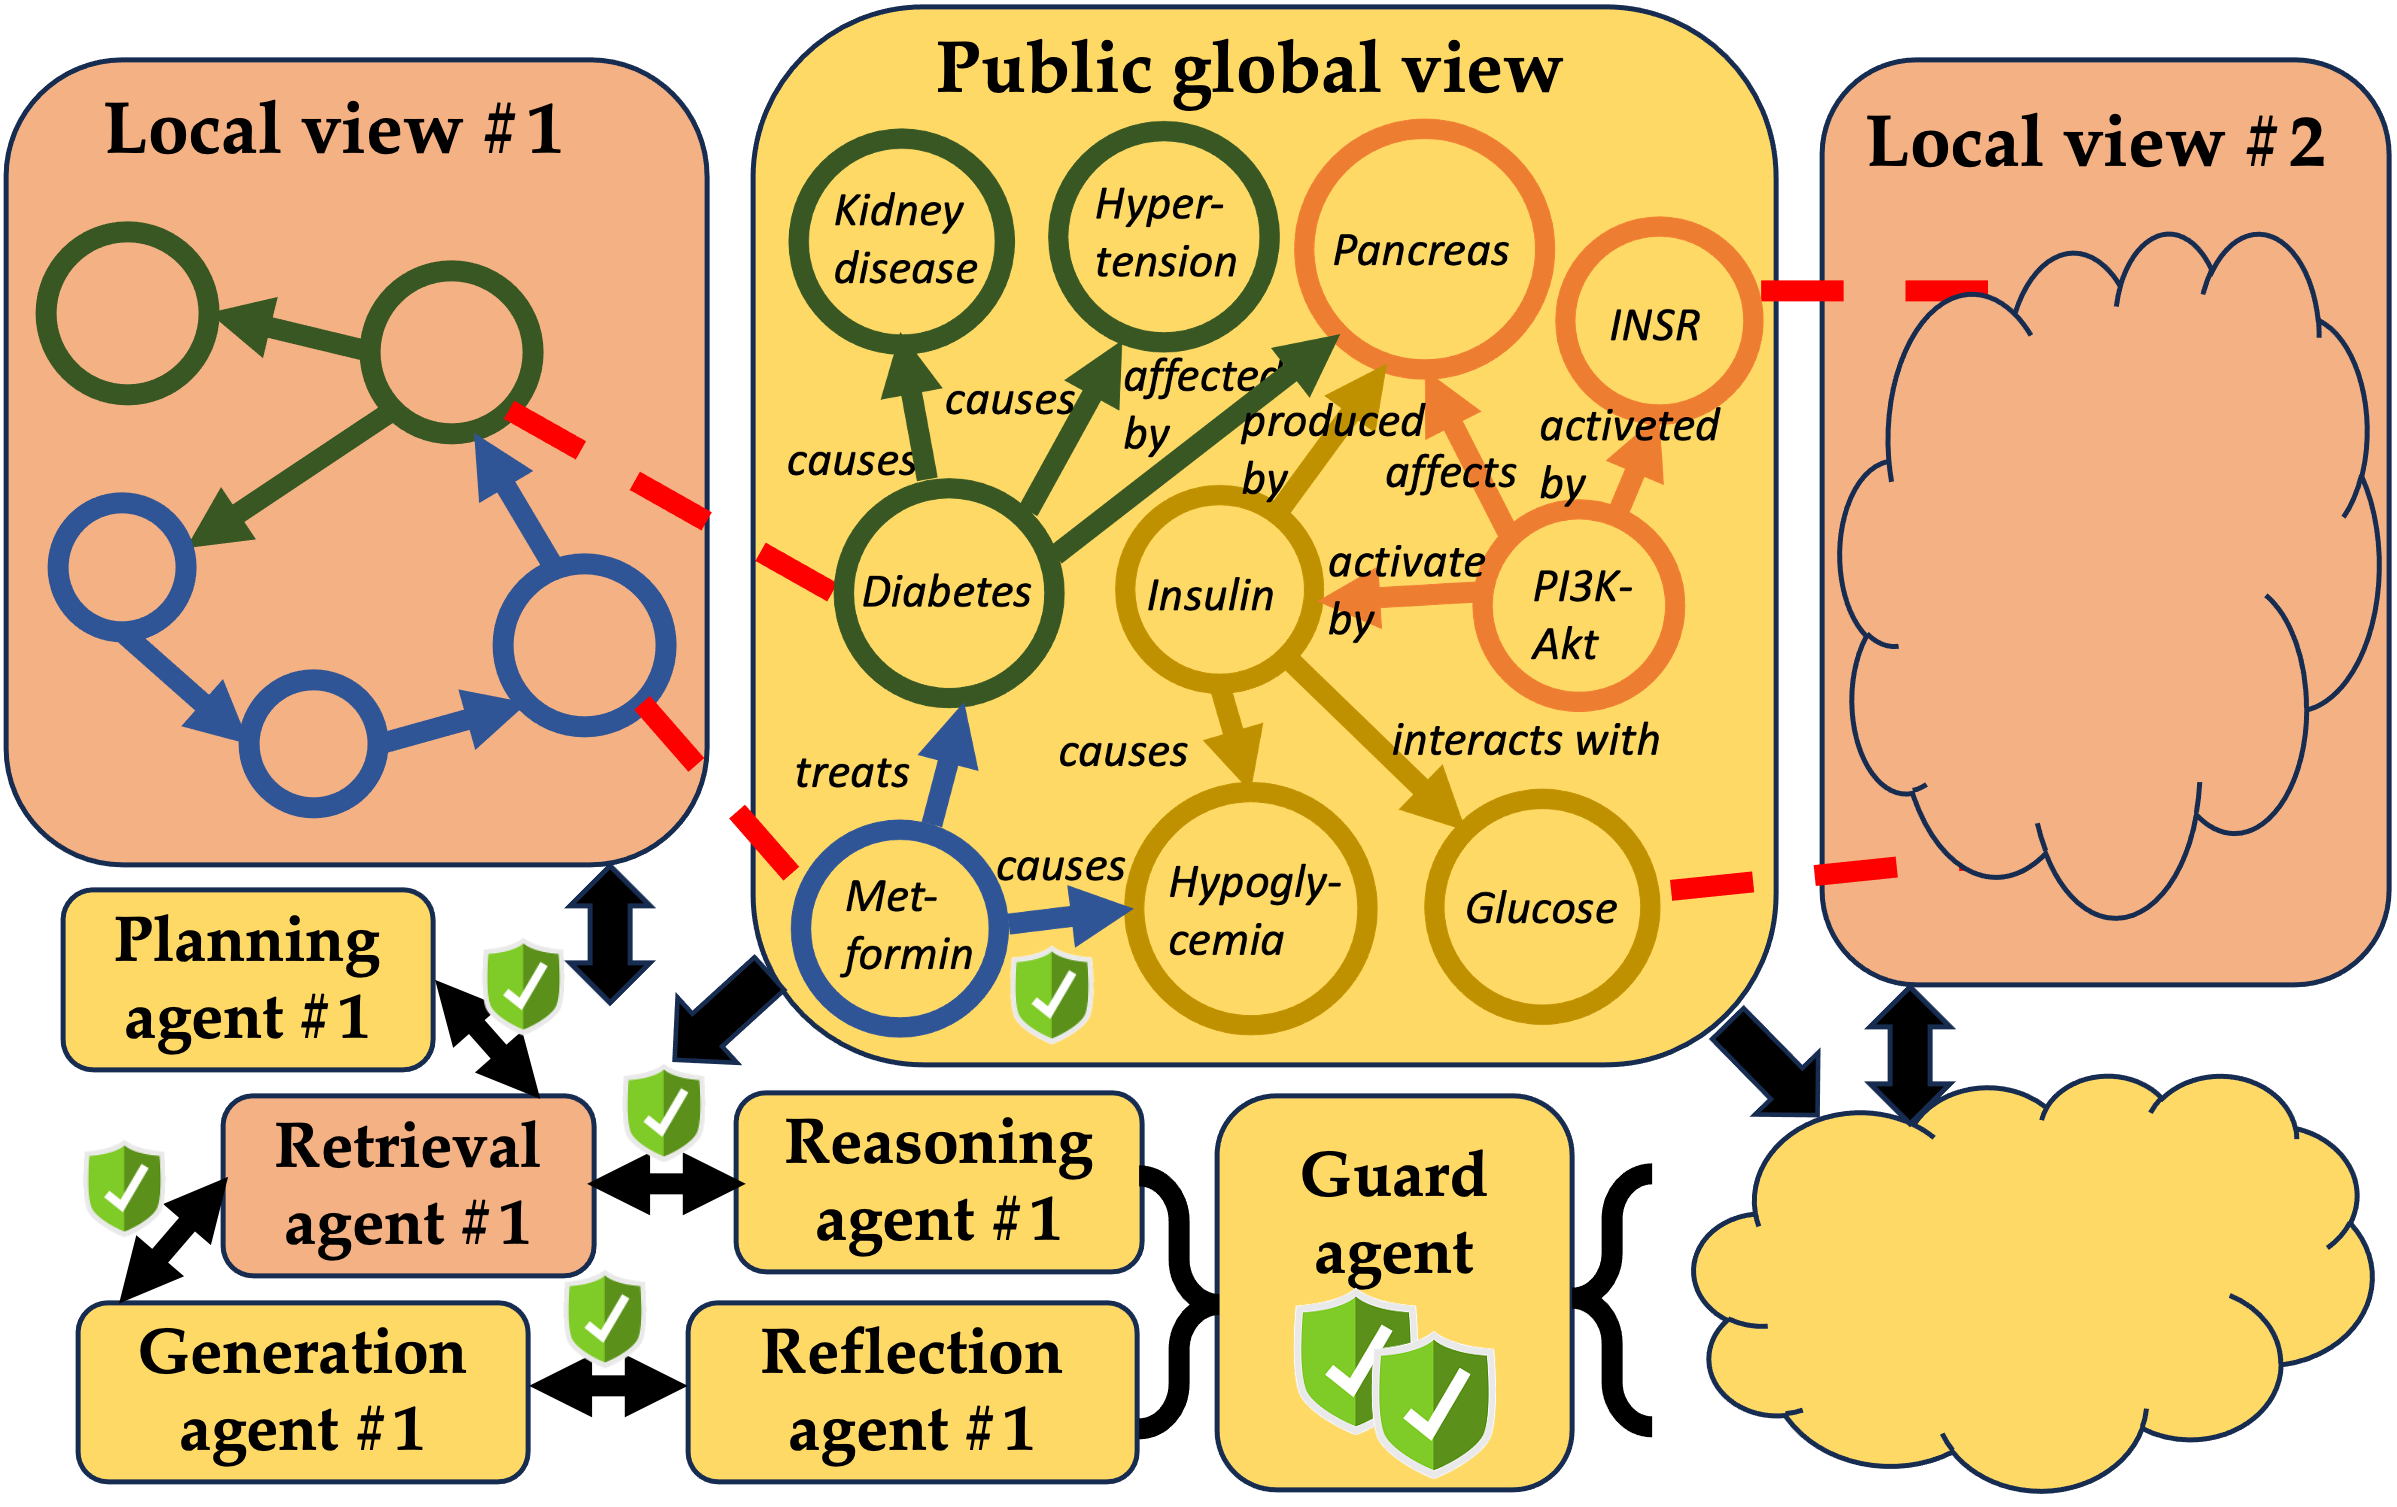
\includegraphics[width=.75\columnwidth]{submissions/CarlYang2024/figures/fedmas.png}
    \end{center}
    % \vspace{-3mm}
    \caption{The envisioned framework of a federated multi-agent system (FedMAS).}
    \label{fig:fedmas}
    % \vspace{-5mm}
\end{figure}

As illustrated in Figure \ref{fig:fedmas}, our envisioned FedMAS will include a multi-view KG and various LLM agents. The federation on KG will be implemented by collectively constructing a multi-view KG by all participating sites, where knowledge from public resources is integrated into the global view, and knowledge from private resources is kept in each site's local view only visible to itself. For each site, entities in its local view are linked with the global view, and only the embeddings related to these linked entities are shared with the server and other sites, via privacy-guaranteed embedding sharing algorithms such as those developed in FedDEP \cite{zhang2024deep} and FedR \cite{zhang2022efficient}. In this way, each local site can compute embeddings on its local view and the public view as if they can see all other sites' local views, allowing them to effectively adjust their local knowledge and further enhance their local LLMs, all without actually seeing the other sites' local views (knowledge). The server will periodically adjust knowledge in the global view also based on the shared privacy-guaranteed embeddings, and apply additional privacy checks to make sure no sensitive knowledge gets propagated into the global view.
%potentially discussing why knowledge is less private and how to avoid inference attack on embeddings

To rigorously protect the more sensitive patient data during the federation on LLM, it is possible to train multiple LLM agents in each site with different functions and let them collaborate through conversations instead of traditional model sharing, so the system can strictly control the level of private data each agent can access and monitor or moderate their collaborations. 
%Based on this design of multi-view KG, we will further enable the federation on LLM by training multiple LLM agents in each site and let them collaborate inside and across sites through conversations. 
%To control the levels of private data access and facilitate the moderation of conversations, each site will train multiple LLM agents focusing on different functions such as planning, retrieval, reasoning, reflection and answer generation. Since all agents will access certain levels of local private data during training and inference, none of them can be directly trained across sites even through FL. To this end, we will build on AutoGen \cite{} to design a structured conversational environment for multi-agent collaboration of LLMs. 
Specifically, since the retrieval agents need to access all local patient data, one plan is to implement programmable guardrails \cite{rebedea2023nemo} on its conversations with all other agents within the same site and forbid them from directly communicating with agents from other sites. Since all other agents can only access patient data indirectly through the retrieval agents, it is possible to adapt techniques such as our recently developed GuardAgent \cite{xiang2024guardagent} based on the clear goals and typical outputs of each agent to monitor all cross-site conversations, detecting and removing any suspicious private information.
%Specifically, since the retrieval and generation agents can directly access local patient data, we will only enable strict one-way conversations from other agents to them; since the planning, reasoning and reflection agents only access local KGs and their performances can likely benefit from cross-site collaborations (such as due to richer knowledge access and more generalized capabilities), we will enable two-way conversations among them cross sites; when the system is normal, we do not expect the agents to ask or answer privacy sensitive questions, and since each agent has clear goals, it will also be relatively easy to detect abnormal conversations; we will also explore techniques such as DP-prompting \cite{} to moderate the conversations against privacy leakage, and conduct red teaming \cite{} to rigorously monitor the conversations.  

When applying FedMAS to specific application domains such as finance, law, education, and healthcare, it is promising to leverage the knowledge-based data sharing mechanism to incorporate existing domain knowledge towards further alleviating knowledge gaps and mitigating potential biases. 
Built on recent promising results from LLM-based data annotations as discussed in Section 2, FedMAS can utilize specialized LLM agents to perform comprehensive extraction of structured knowledge from existing guidelines and tutorials and automatically integrate them with existing general and domain-specific KGs. For example, in healthcare, one type of important domain-specific entity is social determinants of health (SDOH) \cite{artiga2020disparities, artiga2018beyond, who2008closing}. The system can start with a set of known SDOH such as defined by WHO \cite{marmot2005social, phelan2010social}, and further extend the set and discover their impacts and relationships with various risk factors by investigating relevant healthcare literature. The KGs enhanced through these steps are supposed to facilitate the alleviation of various health disparities when utilized by subsequent LLM agents in the FedMAS. 
%Specifically, we will (1) adapt techniques in Thrust 1 with a focus on identifying SDOH-related entities and relations, such as by using the key factors in Figure \ref{fig:t3-3} to create an initial SDOH ontology and using LLMs for its further expansion to include more fine-grained factors; (2) conduct controlled experiments by finding and synthesizing pairs of patient data which only differ by certain SDOH factors, and analyzing LLM outputs for them regarding different clinical questions; (3) based on insights from (2), design programmable guardrails \cite{rebedea2023nemo} to enforce LLMs to output SDOH-removed predictions for tasks such as disease diagnosis where fairness is concerned, and output SDOH-informed predictions for tasks such as treatment suggestion where patients' financial abilities and access to healthcare resources should be considered.

While FedMAS utilizes AI advances to automate multi-site data integration and modeling, comprehensive and trustworthy AI systems need to also incorporate the values and needs of various stakeholders, who can have different and even contradictory perspectives. LLMs, especially in our multi-agent conversational environment, provide unique convenience for effective and efficient human participation, where different stakeholders can verify, influence, and complement the decision processes and outputs of different LLM agents, all based on natural languages as the interface.
Specifically, we envision a novel multi-stage intervention mechanism to efficiently enable the participation of different stakeholders in the LLM-based multi-agent conversational environment. The potential stages could include (1) LLM uncertainty quantification, where LLMs highlight their own uncertain outputs; (2) Rubrics-based rating, where humans create rubrics to automatically rate the LLM outputs; (3) Focused human interactions, where humans directly interact with LLMs, focusing on the problematic scenarios identified in the previous stages. The overall multi-stage mechanism is supposed to allow FedMAS to adapt to human values through iteratively integrating the language-based feedback via interactions with various stakeholders. 

%Instead of having the stakeholders freely chat with LLM agents, the mechanism will work as follows: Stage-1 (Uncertainty): LLM uncertainty quantification methods \cite{farquhar2024detecting, lu2024uncertainty} will be performed to identify potentially problematic answers such as due to hallucinations or data biases; Stage-2 (Rubrics): Rubrics manually generated from stakeholder feedback on a small development set such as based on the guidelines in Figure \ref{fig:t3-2} will be applied to automatically rate new LLM outputs, further exploring or highlighting problematic answers. Stage-3 (Human): Limited and costly human interactions will focus on problematic LLM outputs detected through the previous stages; %, either (partially) following the feedback guidelines or through free-form conversations; the stakeholders will also participate in elaborated surveys after interactions with LLMs, to summarize thoughts and concerns. On a development set, we will have the three stages cross-validate each other to evaluate their individual effectiveness and uncover potentially missed problematic LLM outputs in each individual stage. The uncertainty measurements, rubrics and feedback guidelines will be revised iteratively after the stakeholder surveys and cross-stage validations.

\section{Conclusions and Future Directions}
% \carl{Shirui, can you start helping with this section?}

In this paper, we discuss the trending efforts of co-learning KGs and LLMs. Through the lens of SRAG, we showcase promising attempts to utilize LLMs to automate the construction, integration, and enrichment of KGs, and discuss how KGs can help with planning paths, guide reasoning with structure, and ground knowledge with reflection, enhancing the reliability of LLMs for downstream tasks. We also envision a novel system of multiple agents collaborating in a conversational federated learning environment based on the knowledge-infused, human-engaged LLMs. While the co-learning of KGs and LLMs holds great potential, we envision several promising directions especially from the SRAG perspective.

\paragraph{Effective evaluation of LLM-generated knowledge.}
To achieve effective knowledge enrichment for KGs with LLMs, it is critical to evaluate and guarantee the quality of added and/or modified knowledge. However, new knowledge is hard to evaluate in nature due to the lack of ground truth. Exhaustive human evaluation is costly, but LLMs can be utilized to lubricate the collaboration between humans and machines toward efficient new knowledge evaluation. For example, humans can create guidelines and rubrics for LLMs to screen and rate the new knowledge from different perspectives. LLMs can also evaluate the quality of knowledge with confidence or uncertainty quantifications. Humans can then focus on the LLM-flagged suspicious or uncertain new knowledge to conduct close manual evaluation. 

\paragraph{Unified versus specialized KGs.}
Due to the diversity and breadth of knowledge, it might be difficult to integrate all knowledge into a single unified KG, which might potentially harm the knowledge integrity. As a potential alternative, it may become practical to construct specialized KGs depending on the knowledge needs of different applications. It then remains an open problem regarding how to measure the relevance of knowledge with respect to specific applications and decide what to include/exclude from the specialized KGs.

\paragraph{More powerful KGs.}
Current KGs mostly include general, binary, and pair-wise relations. However, when KGs are used in certain applications, the knowledge may not equally hold for every context. For example, one drug may treat a disease for only certain groups of patients. In such scenarios, specific mechanisms are needed to model the various contexts for knowledge. Moreover, relations are not always binary and pair-wise (between pairs of entities). They can be true with a probability and involve more than two entities. Such scenarios are ubiquitous in reality, so probabilistic KGs and n-ary KGs should receive wider adoption and study.


\paragraph{Trade-off between effectiveness and efficiency of retrieval.}
Most existing retrieval-based methods focus on developing an effective retrieval mechanism to accurately retrieve relevant knowledge from KGs \cite{li2023graph,yang2024kg}. However, they often overlook the efficiency of the retrieval process. In practice, the retrieval process can be computationally expensive, especially when the KG is large. Meanwhile, real-world application often requires prompt responses, which further exacerbates the efficiency issue. Therefore, it is essential to strike a balance between the effectiveness and efficiency of the retrieval process \cite{dehghan-etal-2024-ewek}.

\paragraph{Resolving knowledge conflicts (internal LLM knowledge versus external knowledge).}
LLMs contain a vast amount of knowledge obtained via pre-training. However, the knowledge might be inaccurate or outdated, which could conflict with the knowledge retrieved from KGs \cite{xu2024knowledge}. To resolve the conflict, SPARE \cite{zhao2024steering} utilizes the internal activations of LLMs to identify the conflict. AstuteRAG \cite{wang2024astute} uses a novel RAG approach to adaptively elicit LLM internal knowledge and iteratively consolidate internal and external knowledge. Despite the attempts, how to effectively identify and resolve the conflict between the internal knowledge of LLMs and the external knowledge retrieved from KGs remains an open problem.

\paragraph{Retrieval from multi-modal data.}
KGs store knowledge in diverse modalities such as text, image, and video \cite{zhu2022multi}. Existing KG retrieval methods mainly focus on retrieving textual knowledge. However, the retrieval from multi-modal data is still under-explored. Knowledge from different modalities can complement each other, which could potentially enhance the retrieval performance. Therefore, it is essential to develop retrieval methods that can effectively retrieve knowledge from multi-modal data \cite{long2024generative}.

\paragraph{Robustness/safety of SRAG for LLMs.} 
The safety and robustness of LLMs are receiving increasing attention due to their critical role in developing trustworthy AI systems. Previous research has primarily focused on attacking the LLMs themselves \cite{kumar2023certifying}. However, integrating LLMs with KG retrieval systems expands the attack surface. Attackers could manipulate KGs and the retrieval systems to mislead LLMs, potentially leading to severe consequences \cite{cheng2024trojanrag}. Therefore, enhancing the robustness and safety of the combined KG and LLM systems is an important research direction.

%The attack surface of KGs + LLMs system is enlarged compared with normal LLM systems. How to enhance the robustness and safety of these systems remains an open question \cite{li2024robustness}.
% The attack surface of KGs + LLMs system is enlarged compared with normal LLM systems. How to enhance the robustness and safety of these systems?



\section*{Acknowledgements}
This research was partially supported by the National Science Foundation under Award Number 2319449 and Award Number 2312502, as well as the National Institute Of Diabetes And Digestive And Kidney Diseases of the National Institutes of Health under Award Number K25DK135913. Any opinions, findings, and conclusions or recommendations expressed herein are those of the authors and do not necessarily represent the views, either expressed or implied, of the National Science Foundation, National Institutes of Health, or the U.S. government.
The authors wish to thank the editors and reviewers for their valuable efforts and suggestions.  

%% \ackrule

\bibliographystyle{IEEEtran} 
\bibliography{submissions/CarlYang2024/carlyang,submissions/CarlYang2024/linhao}

%\section*{Biographies}

%\textbf{P. W. Wachulak} received the degree${\ldots}$ \\[6pt]
%\textbf{M. C. Marconi} received the degree${\ldots}$ \\[6pt]
%\textbf{R. A. Bartels} received the degree${\ldots}$ \\[6pt]
%\textbf{C. S. Menoni} received the degree${\ldots}$ \\[6pt]
%\textbf{J. J. Rocca} received the degree${\ldots}$



\end{document}